%%%%%%%%%%%%%%%%%%%%%%%%%%%%%%%%%%%%%%%%%%%%%%%%%%%%%%%%%%%%%%%%%%%%%%%%%%%%
%DIF LATEXDIFF DIFFERENCE FILE
%DIF DEL agutmpl.tex         Mon Mar 20 17:48:59 2017
%DIF ADD revised-draft.tex   Tue Jun  6 15:17:07 2017
% AGUtmpl.tex: this template file is for articles formatted with LaTeX2e,
% Modified March 2013
%
% This template includes commands and instructions
% given in the order necessary to produce a final output that will
% satisfy AGU requirements.
%
% PLEASE DO NOT USE YOUR OWN MACROS
% DO NOT USE \newcommand, \renewcommand, or \def.
%
% FOR FIGURES, DO NOT USE \psfrag or \subfigure.
%
%%%%%%%%%%%%%%%%%%%%%%%%%%%%%%%%%%%%%%%%%%%%%%%%%%%%%%%%%%%%%%%%%%%%%%%%%%%%
%
% All questions should be e-mailed to latex@agu.org.
%
%%%%%%%%%%%%%%%%%%%%%%%%%%%%%%%%%%%%%%%%%%%%%%%%%%%%%%%%%%%%%%%%%%%%%%%%%%%%
%
% Step 1: Set the \documentclass
%
% There are two options for article format: two column (default)
% and draft.
%
% PLEASE USE THE DRAFT OPTION TO SUBMIT YOUR PAPERS.
% The draft option produces double spaced output.
%
% Choose the journal abbreviation for the journal you are
% submitting to:

% jgrga JOURNAL OF GEOPHYSICAL RESEARCH
% gbc   GLOBAL BIOCHEMICAL CYCLES
% grl   GEOPHYSICAL RESEARCH LETTERS
% pal   PALEOCEANOGRAPHY
% ras   RADIO SCIENCE
% rog   REVIEWS OF GEOPHYSICS
% tec   TECTONICS
% wrr   WATER RESOURCES RESEARCH
% gc    GEOCHEMISTRY, GEOPHYSICS, GEOSYSTEMS
% sw    SPACE WEATHER
% ms    JAMES
% ef    EARTH'S FUTURE
%
%
%
% (If you are submitting to a journal other than jgrga,
% substitute the initials of the journal for "jgrga" below.)

\documentclass[sw, draft]{AGUTeX}

\usepackage{amsmath}
\usepackage{txfonts}
\usepackage{graphicx}
\usepackage{booktabs}
\usepackage{url}
\usepackage{lineno}
\linenumbers*[1]
\usepackage{rotating}
\usepackage{adjustbox}
\graphicspath{{figures/}}
%  To add line numbers to lines with equations:
%  \begin{linenomath*}
%  \begin{equation}
%  \end{equation}
%  \end{linenomath*}
%%%%%%%%%%%%%%%%%%%%%%%%%%%%%%%%%%%%%%%%%%%%%%%%%%%%%%%%%%%%%%%%%%%%%%%%%
% Figures and Tables
%
%
% DO NOT USE \psfrag or \subfigure commands.
%
%  Figures and tables should be placed AT THE END OF THE ARTICLE,
%  after the references.
%
%  Uncomment the following command to include .eps files
%  (comment out this line for draft format):
%  \usepackage[dvips]{graphicx}
%
%  Uncomment the following command to allow illustrations to print
%   when using Draft:
  \setkeys{Gin}{draft=false}
%
% Substitute one of the following for [dvips] above
% if you are using a different driver program and want to
% proof your illustrations on your machine:
%
% [xdvi], [dvipdf], [dvipsone], [dviwindo], [emtex], [dviwin],
% [pctexps],  [pctexwin],  [pctexhp],  [pctex32], [truetex], [tcidvi],
% [oztex], [textures]
%
% See how to enter figures and tables at the end of the article, after
% references.
%
%% ------------------------------------------------------------------------ %%
%
%  ENTER PREAMBLE
%
%% ------------------------------------------------------------------------ %%

% Author names in capital letters:
\authorrunninghead{CHANDORKAR ET AL.}

% Shorter version of title entered in capital letters:
\titlerunninghead{GAUSSIAN PROCESS $Dst$ MODELS}

%Corresponding author mailing address and e-mail address:
\authoraddr{Corresponding author: M. H. Chandorkar,
Multiscale Dynamics, Centrum Wiskunde Informatica, Science Park 123, 1098XG Amsterdam, Netherlands.
(mandar.chandorkar@cwi.nl)}
%DIF PREAMBLE EXTENSION ADDED BY LATEXDIFF
%DIF UNDERLINE PREAMBLE %DIF PREAMBLE
\RequirePackage[normalem]{ulem} %DIF PREAMBLE
\RequirePackage{color}\definecolor{RED}{rgb}{1,0,0}\definecolor{BLUE}{rgb}{0,0,1} %DIF PREAMBLE
\providecommand{\DIFadd}[1]{{\protect\color{blue}\uwave{#1}}} %DIF PREAMBLE
\providecommand{\DIFdel}[1]{{\protect\color{red}\sout{#1}}}                      %DIF PREAMBLE
%DIF SAFE PREAMBLE %DIF PREAMBLE
\providecommand{\DIFaddbegin}{} %DIF PREAMBLE
\providecommand{\DIFaddend}{} %DIF PREAMBLE
\providecommand{\DIFdelbegin}{} %DIF PREAMBLE
\providecommand{\DIFdelend}{} %DIF PREAMBLE
%DIF FLOATSAFE PREAMBLE %DIF PREAMBLE
\providecommand{\DIFaddFL}[1]{\DIFadd{#1}} %DIF PREAMBLE
\providecommand{\DIFdelFL}[1]{\DIFdel{#1}} %DIF PREAMBLE
\providecommand{\DIFaddbeginFL}{} %DIF PREAMBLE
\providecommand{\DIFaddendFL}{} %DIF PREAMBLE
\providecommand{\DIFdelbeginFL}{} %DIF PREAMBLE
\providecommand{\DIFdelendFL}{} %DIF PREAMBLE
\newcommand{\DIFscaledelfig}{0.5}
%DIF HIGHLIGHTGRAPHICS PREAMBLE %DIF PREAMBLE
\RequirePackage{settobox} %DIF PREAMBLE
\RequirePackage{letltxmacro} %DIF PREAMBLE
\newsavebox{\DIFdelgraphicsbox} %DIF PREAMBLE
\newlength{\DIFdelgraphicswidth} %DIF PREAMBLE
\newlength{\DIFdelgraphicsheight} %DIF PREAMBLE
% store original definition of \includegraphics %DIF PREAMBLE
\LetLtxMacro{\DIFOincludegraphics}{\includegraphics} %DIF PREAMBLE
\newcommand{\DIFaddincludegraphics}[2][]{{\color{blue}\fbox{\DIFOincludegraphics[#1]{#2}}}} %DIF PREAMBLE
\newcommand{\DIFdelincludegraphics}[2][]{% %DIF PREAMBLE
\sbox{\DIFdelgraphicsbox}{\DIFOincludegraphics[#1]{#2}}% %DIF PREAMBLE
\settoboxwidth{\DIFdelgraphicswidth}{\DIFdelgraphicsbox} %DIF PREAMBLE
\settoboxtotalheight{\DIFdelgraphicsheight}{\DIFdelgraphicsbox} %DIF PREAMBLE
\scalebox{\DIFscaledelfig}{% %DIF PREAMBLE
\parbox[b]{\DIFdelgraphicswidth}{\usebox{\DIFdelgraphicsbox}\\[-\baselineskip] \rule{\DIFdelgraphicswidth}{0em}}\llap{\resizebox{\DIFdelgraphicswidth}{\DIFdelgraphicsheight}{% %DIF PREAMBLE
\setlength{\unitlength}{\DIFdelgraphicswidth}% %DIF PREAMBLE
\begin{picture}(1,1)% %DIF PREAMBLE
\thicklines\linethickness{2pt} %DIF PREAMBLE
{\color[rgb]{1,0,0}\put(0,0){\framebox(1,1){}}}% %DIF PREAMBLE
{\color[rgb]{1,0,0}\put(0,0){\line( 1,1){1}}}% %DIF PREAMBLE
{\color[rgb]{1,0,0}\put(0,1){\line(1,-1){1}}}% %DIF PREAMBLE
\end{picture}% %DIF PREAMBLE
}\hspace*{3pt}}} %DIF PREAMBLE
} %DIF PREAMBLE
\LetLtxMacro{\DIFOaddbegin}{\DIFaddbegin} %DIF PREAMBLE
\LetLtxMacro{\DIFOaddend}{\DIFaddend} %DIF PREAMBLE
\LetLtxMacro{\DIFOdelbegin}{\DIFdelbegin} %DIF PREAMBLE
\LetLtxMacro{\DIFOdelend}{\DIFdelend} %DIF PREAMBLE
\DeclareRobustCommand{\DIFaddbegin}{\DIFOaddbegin \let\includegraphics\DIFaddincludegraphics} %DIF PREAMBLE
\DeclareRobustCommand{\DIFaddend}{\DIFOaddend \let\includegraphics\DIFOincludegraphics} %DIF PREAMBLE
\DeclareRobustCommand{\DIFdelbegin}{\DIFOdelbegin \let\includegraphics\DIFdelincludegraphics} %DIF PREAMBLE
\DeclareRobustCommand{\DIFdelend}{\DIFOaddend \let\includegraphics\DIFOincludegraphics} %DIF PREAMBLE
\LetLtxMacro{\DIFOaddbeginFL}{\DIFaddbeginFL} %DIF PREAMBLE
\LetLtxMacro{\DIFOaddendFL}{\DIFaddendFL} %DIF PREAMBLE
\LetLtxMacro{\DIFOdelbeginFL}{\DIFdelbeginFL} %DIF PREAMBLE
\LetLtxMacro{\DIFOdelendFL}{\DIFdelendFL} %DIF PREAMBLE
\DeclareRobustCommand{\DIFaddbeginFL}{\DIFOaddbeginFL \let\includegraphics\DIFaddincludegraphics} %DIF PREAMBLE
\DeclareRobustCommand{\DIFaddendFL}{\DIFOaddendFL \let\includegraphics\DIFOincludegraphics} %DIF PREAMBLE
\DeclareRobustCommand{\DIFdelbeginFL}{\DIFOdelbeginFL \let\includegraphics\DIFdelincludegraphics} %DIF PREAMBLE
\DeclareRobustCommand{\DIFdelendFL}{\DIFOaddendFL \let\includegraphics\DIFOincludegraphics} %DIF PREAMBLE
%DIF END PREAMBLE EXTENSION ADDED BY LATEXDIFF

\begin{document}

%% ------------------------------------------------------------------------ %%
%
%  TITLE
%
%% ------------------------------------------------------------------------ %%


\title{Probabilistic Forecasting of the Disturbance Storm Time Index: An Autoregressive Gaussian Process approach}

\authors{M. Chandorkar,\altaffilmark{1}
 E. Camporeale,\altaffilmark{1}
 S. Wing\altaffilmark{2}}

\altaffiltext{1}{Multiscale Dynamics, Centrum Wiskunde Informatica (CWI), Amsterdam,
              1098XG Amsterdam}

\altaffiltext{2}{The Johns Hopkins University Applied Physics Laboratory, 
              Laurel, Maryland, 20723, USA}

% >> Do NOT include any \begin...\end commands within
% >> the body of the abstract.

\begin{abstract}
We present a methodology for generating probabilistic predictions for the \emph{Disturbance Storm Time} ($Dst$) geomagnetic activity index. We focus on the \emph{One Step Ahead} (OSA) prediction task and use the OMNI hourly resolution data to build our models.

Our proposed methodology is based on the technique of \emph{Gaussian Process Regression} (GPR). Within this framework we develop two models; \emph{Gaussian Process Auto-Regressive} (GP-AR) and \emph{Gaussian Process Auto-Regressive with eXogenous inputs} (GP-ARX). 

We also propose a criterion to aid model selection with respect to the order of auto-regressive inputs. Finally we test the performance of the GP-AR and GP-ARX models on a set of 63 geomagnetic storms between 1998 and 2006 and illustrate sample predictions with error bars for some of these events.

\end{abstract}

%% ------------------------------------------------------------------------ %%
%
%  BEGIN ARTICLE
%
%% ------------------------------------------------------------------------ %%

% The body of the article must start with a \begin{article} command
%
% \end{article} must follow the references section, before the figures
%  and tables.

\begin{article}

%% ------------------------------------------------------------------------ %%
%
%  TEXT
%
%% ------------------------------------------------------------------------ %%

\section{Introduction}


The magnetosphere's dynamics and its associated solar wind driver form a complex dynamical system. It is therefore instructive and greatly simplifying to use representative indices to quantify the state of geomagnetic activity.

Geomagnetic indices come in various forms, they may take continuous or discrete values and may be defined with varying time resolutions. Their values are often calculated by averaging or combining a number of readings taken by instruments, usually magnetometers, around the Earth. Each geomagnetic index is a proxy for a particular kind of phenomenon. Some popular indices are the $K_p$, $Dst$ and the $AE$ index.

\begin{enumerate}
    \item $K_p$: The Kp-index is a discrete valued global geomagnetic activity index and is based on 3 hour measurements of the K-indices \citep{Bartels}. The K-index itself is a three hour long quasi-logarithmic local index of the geomagnetic activity, relative to a calm day curve for the given location.

    \item $AE$: The Auroral Electrojet Index, $AE$, is designed to provide a global, quantitative measure of auroral zone magnetic activity produced by enhanced Ionospheric currents flowing below and within the auroral oval \citep{AEIndex}. It is a continuous index which is calculated every hour.

    \item $Dst$: A continuous hourly index which gives a measure of the weakening or strengthening of the Earth's equatorial magnetic field due to \DIFdelbegin \DIFdel{the }\DIFdelend \DIFaddbegin \DIFadd{particle injection in the magnetosphere. Particle injection has a number of sources such as, }\DIFaddend weakening or strengthening of the ring currents and the geomagnetic storms \citep{DesslerAndParker}\DIFaddbegin \DIFadd{, near Earth cross tail current \mbox{%DIFAUXCMD
\citep{ganushkina2004long} }%DIFAUXCMD
and \mbox{%DIFAUXCMD
\citep{angeo-28-123-2010}}%DIFAUXCMD
, partial ring current \mbox{%DIFAUXCMD
\citep{JGRA:JGRA15878}}%DIFAUXCMD
, substorm current wedge \mbox{%DIFAUXCMD
\citep{JGRA:JGRA15211}}%DIFAUXCMD
, magnetopause current, etc }\DIFaddend . 
\end{enumerate}

%Talk about Burton and friends
For the present study, we focus on prediction of the hourly $Dst$ index which is a straightforward indicator of geomagnetic storms. More specifically, we focus on the \emph{one step ahead} (OSA) (in this case one hour ahead) prediction of $Dst$ because it is the simplest model towards building long term predictions of geomagnetic response of the Earth to changing space weather conditions. 

The $Dst$ OSA prediction problem has been the subject of several modeling efforts in the literature. One of the earliest models has been presented by \citet{JGR:JGR10260} who calculated $Dst(t)$ as the solution of an \emph{Ordinary Differential Equation} (ODE) which expressed the rate of change of $Dst(t)$ as a combination of two terms: decay and injection $\frac{d Dst(t)}{dt} = Q(t) - \frac{Dst(t)}{\tau}$, where $Q(t)$ relates to the particle injection from the plasma sheet into the inner magnetosphere. 

The \citet{JGR:JGR10260} model has proven to be very influential particularly due to its simplicity. Many subsequent works have modified the proposed ODE by proposing alternative expressions for the injection term $Q(t)$ [see \citet{Wang:Dst}, \citet{JGRA:JGRA14856}]. More recently \citet{Ballatore2014} have tried to generate empirical estimates for the injection and decay terms in Burton's equation.

%Talk about NARMAX Dst
Another important empirical model used to predict $Dst$ is the \emph{Nonlinear Auto-Regessive Moving Average with eXogenous inputs} (NARMAX) methodology developed in \citet{doi:10.1080/00207178908559767}, \citet{GRL:GRL13494}, \citet{GRL:GRL20944}, \citet{JGRA:JGRA18657}, \citet{balikhin:narmax}, \citet{JGRA:JGRA20661} and \citet{JGRA:JGRA50192}. The NARMAX methodology builds models by constructing polynomial expansions of inputs and determines the best combinations of monomials to include in the refined model by using a criterion called the \emph{error reduction ratio} (ERR). The parameters of the so called NARMAX OLS-ERR model are calculated by solving the \emph{ordinary least squares} (OLS) problem arising from a quadratic objective function. \DIFaddbegin \DIFadd{It must be noted that the NARMAX methodology is not limited to polynomial functions, rather any set of basis function expansions can be used with it, such as radial basis functions, wavelets etc \mbox{%DIFAUXCMD
\citep{doi:10.1080/00207720600903011}}%DIFAUXCMD
, \mbox{%DIFAUXCMD
\citep{JGRA:JGRA17327}}%DIFAUXCMD
. }\DIFaddend The reader may refer to \citet{billings2013nonlinear} for a detailed exposition of the NARMAX methodology.

%Talk about neural networks
Yet another family of forecasting methods is based on \emph{Artificial Neural Networks} (ANN) that have been a popular choice for building predictive models. Researchers have employed both the standard \emph{feed forward} and the more specialized \emph{recurrent} architectures. \citet{Lund} proposed an \emph{Elman} recurrent network architecture called Lund $Dst$, which used the solar wind velocity, \emph{interplanetary magnetic field} (IMF) and historical $Dst$ data as inputs. \citet{JGRA:JGRA17461} used recurrent neural networks to predict $Kp$. \citet{SWE:SWE286} originally proposed a \emph{feed forward} network for predicting the $K_p$ index which used the \emph{Boyle coupling function} \citet{boyle1997empirical}. The same architecture is adapted for prediction of $Dst$ in \citet{SWE:SWE286}, popularly known as the Rice $Dst$ model. \citet{pallocchia:hal-00318011} proposed a \emph{neural network} model called EDDA to predict $Dst$ using only the IMF data.

%DIF > Local neurofuzzy modelling and singular spectrum analysis.
\DIFaddbegin \DIFadd{Apart from the NARMAX and neural network approaches, fuzzy methods have also been applied for $Dst$ prediction, \mbox{%DIFAUXCMD
\citet{SWE:SWE146} }%DIFAUXCMD
and \mbox{%DIFAUXCMD
\citet{Sharifi2006} }%DIFAUXCMD
outline the application of }\emph{\DIFadd{Local Neurofuzzy}} \DIFadd{models for one hour and two hour predictions of $Dst$ respectively. Local neuro-fuzzy models reduce the input space into a number of regions each with its own expert predictor. The combined model predicts $Dst$ for a new point as a linear combinations of the predictions from each expert weighted by a fuzzy score signifying the importance of each model for the provided input. For improving predictive performance of two hour $Dst$ forecasts in \mbox{%DIFAUXCMD
\citet{Sharifi2006}}%DIFAUXCMD
, the authors use }\emph{\DIFadd{singular spectrum analysis}} \DIFadd{(SSA). Singular spectrum analysis consists of extracting orthogonal components from a lagged time series, it is equivalent to }\emph{\DIFadd{principal component analysis}} \DIFadd{(PCA) which is quite extensively used in the machine learning community. \mbox{%DIFAUXCMD
\citet{loskutov2001testing} }%DIFAUXCMD
and \mbox{%DIFAUXCMD
\citet{loskutov2001study} }%DIFAUXCMD
provide a good background to the theory and application of SSA to geomagnetic time series.
}

\DIFaddend %Talk about need for probabilistic forecasts.
Although much research has been done on prediction of the $Dst$ index, much less has been done on probabilistic forecasting of $Dst$. One such work described in \citet{McPherron:2013} involves identification of high speed solar wind streams using the WSA model (see \citet{WSAModel}), using predictions of high speed streams to construct ensembles of $Dst$ trajectories which yield the quartiles of $Dst$ time series. 

\DIFaddbegin \DIFadd{A simple way to construct error bars on the predictions of forecasting models is by using the so called }\textit{\DIFadd{past cast}} \DIFadd{performance i.e. by calculating the standard deviations of the predictions generated by the model on a hold out data set. One limitation of such an approach is that the variance of the model predictions is computed once and for all. It does not adapt according to the inputs provided to the model. This may lead to overestimation or underestimation of the uncertainty around a given prediction, depending on the prevelant geo-magnetic conditions and the data set used to calculate the }\textit{\DIFadd{past cast}} \DIFadd{model performance.
}

\DIFaddend In this work we propose a technique for probabilistic forecasting of $Dst$, which yields a predictive distribution as a closed form expression. Our models take as input past values of $Dst$, solar wind speed and the \textit{z} component of the \emph{Interplanetary Magnetic Field} (IMF) and output a Gaussian distribution with a specific mean and variance as the OSA prediction of the $Dst$. 

We use the \emph{Gaussian Process Regression} methodology to construct auto-regressive models for $Dst$ and show how to perform exact inference in this framework. We further outline a methodology to perform model selection with respect to its free parameters and time histories.

The remainder of this paper is organised as follows: Section \ref{sec:method} gives the reader an overview of the history of \emph{Gaussian Process} models as well as how they are formulated and how to perform inference with them. Sections \ref{sec:osa}, \ref{sec:modeltraining} describe the GP-AR and GP-ARX models for OSA prediction of $Dst$ and how to choose their free parameters for better performance. 

\section{Methodology: Gaussian Process} \label{sec:method}

\emph{Gaussian Processes} first appeared in machine learning research in \citet{Neal:1996:BLN:525544}, as the limiting case of Bayesian inference performed on neural networks with infinitely many neurons in the hidden layers. Although their inception in the machine learning community is recent, their origins can be traced back to the geo-statistics research community where they are known as \emph{Kriging} methods (\citet{krige1951statistical}). In pure mathematics area \emph{Gaussian Processes} have been studied extensively and their existence was first proven by Kolmogorov's extension theorem (\citet{tao2011introduction}). The reader is referred to \citet{Rasmussen:2005:GPM:1162254} for an in depth treatment of Gaussian Processes in machine learning.

Let us assume that we want to model a process in which a scalar quantity $y$ is specified as $y = f(\mathbf{x}) + \epsilon$ where   $f(.): \mathbb{R}^d \rightarrow \mathbb{R}$ is an unknown scalar function of a multidimensional input vector $\mathbf{x} \in \mathbb{R}^d$, $d$ is the dimensionality of the input space, and $\epsilon \sim \mathcal{N}(0, \sigma^2)$ is zero mean Gaussian noise with variance $\sigma^2$.

A set of labeled data points ${(\mathbf{x}_i, y_i); i = 1 \cdots N}$ can be conveniently expressed by a $N \times d$ data matrix $\mathbf{X}$ and a $N \times 1$ response vector $\mathbf{y}$, as shown in equations (\ref{eq:feat}) and (\ref{eq:labels}).

\begin{align}
  \mathbf{X}  = & \left( \begin{array}{c} \mathbf{x}^{T}_1 \\ \mathbf{x}^{T}_2 \\ \vdots \\ \mathbf{x}^{T}_N \end{array} \right)_{N \times d} \label{eq:feat} \\
  \vspace{2\baselineskip}
  \mathbf{y}  = & \left( \begin{array}{c} y_1 \\ y_2 \\ \vdots \\ y_N \end{array} \right) _{N \times 1} \label{eq:labels}
\end{align}

Our task is to infer the values of the unknown function $f(.)$ based on the inputs $\mathbf{X}$ and the noisy observations $\mathbf{y}$. We now assume that the joint distribution of $f(\mathbf{x}_i), i = 1 \cdots N$ is a multivariate Gaussian as shown in equations (\ref{eq:fvalues}), (\ref{eq:normal}) and (\ref{eq:sto}).

\begin{align}
 \mathbf{f} = & \left( \begin{array}{c} f(\mathbf{x}_1) \\ f(\mathbf{x}_2) \\ \vdots \\ f(\mathbf{x}_N) \end{array} \right) \label{eq:fvalues}\\
 \vspace{2\baselineskip}
 \mathbf{f} | \mathbf{x}_1, \cdots, \mathbf{x}_N \sim & \mathcal{N}\left( \mathbf{\mu}, \mathbf{\Lambda} \right)  \label{eq:normal}\\
 \vspace{2\baselineskip}
 p( \mathbf{f} \ | \ \mathbf{x}_1, \cdots, \mathbf{x}_N) = & \frac{1}{(2\pi)^{n/2} det(\mathbf{\Lambda})^{1/2}} exp \left(-\frac{1}{2} (\mathbf{f} - \mathbf{\mu})^T \mathbf{\Lambda}^{-1} (\mathbf{f} - \mathbf{\mu}) \right) \label{eq:sto}
\end{align}

Here $\mathbf{f}$ is a $N\times 1$ vector consisting of the values $f(\mathbf{x}_i), i = 1 \cdots N$. In equation (\ref{eq:normal}), $\mathbf{f}|\mathbf{x}_1, \cdots, \mathbf{x}_N$ denotes the conditional distribution of $\mathbf{f}$ with respect to the input data (i.e., $\mathbf{X}$) and $\mathcal{N}\left( \mathbf{\mu}, \mathbf{\Lambda} \right)$ represents a multivariate Gaussian distribution with mean vector $\mathbf{\mu}$ and covariance matrix $\mathbf{\Lambda}$. The probability density function of this distribution $p( \mathbf{f} \ | \ \mathbf{x}_1, \cdots, \mathbf{x}_N)$ is therefore given by equation (\ref{eq:sto}).

From equation (\ref{eq:sto}), one can observe that in order to uniquely define the distribution of the process, it is required to specify $\mathbf{\mu}$ and $\mathbf{\Lambda}$. For this probability density to be valid, there are further requirements imposed on $\mathbf{\Lambda}$: 

\begin{enumerate}
      \item Symmetry: $\mathbf{\Lambda}_{ij} = \mathbf{\Lambda}_{ji} \ \forall i,j \in {1, \cdots, N} $ 
      \item Positive Semi-definiteness: $\mathbf{z}^T \mathbf{\Lambda} \mathbf{z} \geq 0 \ \forall \mathbf{z} \in \mathbb{R}^N$  
\end{enumerate}

Inspecting the individual elements of $\mathbf{\mu}$ and $\mathbf{\Lambda}$, we realise that they take the following form.

\begin{align}
      \mu_i = & \mathbb{E}[f(\mathbf{x}_i)] := m(\mathbf{x}_i) \\
      \Lambda_{ij} = & \mathbb{E}[(f(\mathbf{x}_i) - \mu_i)(f(\mathbf{x}_j) - \mu_j)] := K(\mathbf{x}_i, \mathbf{x}_j)
\end{align}

Here $\mathbb{E}$ denotes the expectation (average). The elements of $\mathbf{\mu}$ and $\mathbf{\Lambda}$ are expressed as functions $m(\mathbf{x}_i)$ and $K(\mathbf{x}_i, \mathbf{x}_j)$ of the inputs $\mathbf{x}_i,\ \mathbf{x}_j$. Specifying the functions $m(\mathbf{x})$ and $K(\mathbf{x}, \mathbf{x}')$ completely specifies each element of $\mathbf{\mu}$ and $\mathbf{\Lambda}$ and subsequently the finite dimensional distribution of $\mathbf{f} | \mathbf{x}_1, \cdots, \mathbf{x}_N $. In most practical applications of \emph{Gaussian Processes} the mean function is often defined as $m(\mathbf{x}) = 0$, which is not unreasonable if the data is standardized to have zero mean. \emph{Gaussian Processes} are represented in machine learning literature using the following notation:

\begin{equation}
    f(\mathbf{x}) \sim \mathcal{GP}(m(\mathbf{x}), K(\mathbf{x}, \mathbf{x}'))
\end{equation}

\subsection{Inference and Predictions} \label{sec:inference}

Our aim is to infer the function $f(\mathbf{x})$ from the noisy training data and generate predictions $f(\mathbf{x}^{*}_i)$ for a set of test points $ {\mathbf{x}^{*}_i : \forall i \in 1, \cdots, M} $. We define $\mathbf{X}^*$ as the test data matrix whose rows are formed by $\mathbf{x}^{*}_i$ as shown in equation (\ref{eq:testfeat}). 
\begin{equation}
    \mathbf{X}_* = \left( \begin{array}{c} (\mathbf{x}^{*}_1)^T \\ (\mathbf{x}^{*}_2)^T \\ \vdots \\ (\mathbf{x}^{*}_M)^T \end{array} \right)_{M \times d} \label{eq:testfeat} 
\end{equation}

Using the multivariate Gaussian distribution in equation (\ref{eq:sto}) we can construct the joint distribution of $f(\mathbf{x})$ over the training and test points. The vector of training and test outputs $\left( \begin{array}{c} \mathbf{y} \\ \mathbf{f_*} \end{array} \right)$ is of dimension $(N+M) \times 1$ and is constructed by appending the test set predictions $\mathbf{f}_*$ to the observed noisy measurements $\mathbf{y}$.

\begin{align}
    \mathbf{f}_* = & \left( \begin{array}{c} f(\mathbf{x^{*}_1}) \\ f(\mathbf{x^{*}_2}) \\ \vdots \\ f(\mathbf{x^{*}_M}) \end{array} \right)_{M \times 1} \\
     \vspace{4\baselineskip}
    \left( \begin{array}{c} \mathbf{y} \\ \mathbf{f_*} \end{array} \right) | \ \ \mathbf{X}, \mathbf{X}_* \sim & 
    \mathcal{N}\left(\mathbf{0}, \left[ \begin{array}{cc} \mathbf{K} + \sigma^{2} \mathbf{I} & \mathbf{K}_{*} \\ \mathbf{K}_{*}^T & \mathbf{K}_{**} \end{array} \right ] \right) \label{eq:dist}
\end{align}

Since we have noisy measurements of $f$ over the training data, we add the noise variance $\sigma^2$ to the variance of $f$ as shown in (\ref{eq:dist}). The block matrix components of the $(N+M) \times (N+M)$ covariance matrix have the following structure.

\begin{enumerate}
      \item $\mathbf{I}$: The $N \times N$ identity matrix.
      \item $\mathbf{K} = [K(\mathbf{x}_i, \mathbf{x}_j)], \ i,j \in 1,\cdots,N$ : Kernel matrix constructed from all couples obtained from the training data.
      \item $\mathbf{K}_{*} = [K(\mathbf{x}_i, \mathbf{x}^{*}_j)], \ i \in 1,\cdots,N ; j \in 1,\cdots,M$ : Cross kernel matrix constructed from all couples between training and test data points.
      \item $\mathbf{K}_{**} = [K(\mathbf{x}^{*}_i, \mathbf{x}^{*}_j)], \ i,j \in 1,\cdots,M$: Kernel matrix constructed from all couples obtained from the test data.
\end{enumerate}

With the multivariate normal distribution defined in equation (\ref{eq:dist}), probabilistic predictions $f_*$ can be generated by constructing the conditional distribution $\mathbf{f_*}|\mathbf{X},\mathbf{y},\mathbf{X_*}$. Since the original distribution of $\left( \begin{array}{c} \mathbf{y} \\ \mathbf{f_*} \end{array} \right) | \ \ \mathbf{X}, \mathbf{X}_*$ is a multivariate Gaussian, conditioning on a subset of elements $\mathbf{y}$ yields another Gaussian distribution whose mean and covariance can be calculated exactly, as in equation (\ref{eq:posterior}) (see \citet{Rasmussen:2005:GPM:1162254}).

\begin{equation}
    \mathbf{f_*}|\mathbf{X},\mathbf{y},\mathbf{X_*} \sim \mathcal{N}(\mathbf{\bar{f}_*}, \Sigma_*)  \label{eq:posterior},
\end{equation}
where
\begin{align}
    \mathbf{\bar{f}_*} = & \mathbf{K}^T_{*} [\mathbf{K} + \sigma^{2} \mathbf{I}]^{-1} \mathbf{y} \label{eq:posteriormean} \\
    \Sigma_* = & \mathbf{K}_{**} - \mathbf{K}^T_{*} \left(\mathbf{K} + \sigma^{2} \mathbf{I}\right)^{-1} \mathbf{K}_{*} \label{eq:posteriorcov}
\end{align}

The practical implementation of \emph{Gaussian Process} models requires the inversion of the training data kernel matrix $[\mathbf{K} + \sigma^{2} \mathbf{I}]^{-1}$ to calculate the parameters of the predictive distribution $\mathbf{f_*}|\mathbf{X},\mathbf{y},\mathbf{X_*}$. The computational complexity of this inference is dominated by the linear problem in Eq. (\ref{eq:posteriormean}), which can be solved via Cholesky decomposition, with a time complexity of $O(N^3)$, where $N$ is the number of data points.

The distribution of $\mathbf{f_*}| \mathbf{X},\mathbf{y},\mathbf{X_*}$ is known in Bayesian analysis as the \emph{Posterior Predictive Distribution}. This illustrates a key difference between \emph{Gaussian Processes} and other regression models such as \emph{Neural Networks}, \emph{Linear Models} and \emph{Support Vector Machines}: a \emph{Gaussian Process} model does not generate point predictions for new data but outputs a predictive distribution for the quantity sought, thus allowing to construct error bars on the predictions. This property of Bayesian models such as \emph{Gaussian Processes} makes them very appealing for Space Weather forecasting applications. 

The central design issue in applying \emph{Gaussian Process} models is the choice of the function $K(\mathbf{x}, \mathbf{x}')$. The same constraints that apply to $\mathbf{\Lambda}$ also apply to the function $K$. In machine learning, these symmetric positive definite functions of two variables are known as \emph{kernels}. Kernel based methods are applied extensively in data analysis i.e. regression, clustering, classification, density estimation (see \citet{Scholkopf:2001:LKS:559923}, \citet{hofmann2008}).

\subsection{Kernel Functions}

For the success of a \emph{Gaussian Process} model an appropriate choice of kernel function is paramount. The symmetry and positive semi-definiteness of \emph{Gaussian Process} kernels implies that they represent inner-products between some basis function representation of the data. The interested reader is suggested to refer to \citet{Berlinet2004}, \citet{Scholkopf:2001:LKS:559923} and \citet{hofmann2008} for a thorough treatment of kernel functions and the rich theory behind them. Some common kernel functions used in machine learning are listed in Table \ref{table:kernel}. 

The quantities $l$ in the RBF, and $b$ and $d$ in the polynomial kernel are known as \emph{hyper-parameters}. Hyper-parameters give flexibility to a particular kernel structure, for example $d = 1, 2, 3, \cdots$ in the polynomial kernel represents linear, quadratic, cubic and higher order polynomials respectively. The process of assigning values to the \emph{hyper-parameters} is crucial in the model building process and is known as \emph{model selection}. 

\subsection{Model Selection}

Given a GP model with a kernel function $K_\theta$, the problem of model selection consists of finding appropriate values for the kernel hyper-parameters $\theta = \left(\theta_1, \theta_2, \cdots, \theta_i\right)$. In order to assign a value to $\theta$, we must define an objective function which represents our confidence that the GP model built from a particular value of $\theta$ is the best performing model. Since GP models encode assumptions about the probability distribution of the output data $\mathbf{y}$ given inputs $\mathbf{X}$, it is natural to use the negative log-likelihood of the training data as a model selection criterion. 

\begin{align*}
  Q(\theta) & = - log(p(\mathbf{y}|\mathbf{X}, K_\theta)) \\
            & = -\frac{1}{2} \mathbf{y}^\intercal (\mathbf{K}_\theta + \sigma^{2} \mathbf{I})^{-1} \mathbf{y} - \frac{1}{2}|\mathbf{K}_\theta + \sigma^{2} \mathbf{I}| - \frac{N}{2}log(2\pi) \\
  \mathbf{K}_\theta & = [K_{\theta}(\mathbf{x}_i, \mathbf{x}_j)]_{N \times N}
\end{align*}

The model selection problem can now be expressed as the minimization problem shown below.

\begin{align*}
\theta^* = arg\min_{\theta} \ Q(\theta)
\end{align*}

The objective function $Q(\theta)$ in the general case can have multiple local minima, and evaluating the value of $Q(.)$ at any given $\theta$ requires inversion of the matrix $\mathbf{K}_\theta + \sigma^{2} \mathbf{I}$ which has a time complexity $O(N^3)$ as noted above. In the interest of saving computational cost, one cannot use exhaustive search through the domain of the hyper-parameters to inform our choice for $\theta$. Some of the techniques used for model selection in the context of GPR include.

\begin{enumerate}
\item Grid Search: Construct a grid of values for $\theta$ as the cartesian product of one dimensional grids for each $\theta_i$, evaluate $Q(.)$ at each such grid point and choose the configuration which yields minimum value of $Q(.)$.

\item Coupled Simulated Annealing: Introduced in \citet{Xavier-De-Souza2010}, it follows the same procedure as \emph{grid search}, but after evaluation of the objective $Q(.)$ on the grid, each grid point is iteratively mutated in a random walk fashion. This mutation is accepted or rejected according to the new value of $Q(.)$ as well as its value on the other grid points. This procedure is iterated until some stop criterion is reached.

\item Maximum Likelihood: This technique as outlined in \citet{Rasmussen:2005:GPM:1162254} is a form of \emph{gradient descent}. It involves starting with an initial guess for $\theta$ and iteratively improving it by calculating the gradient of $Q(.)$ with respect to $\theta$. Although this method seems intuitive, it introduces an extra computational cost of calculating the gradient of $Q(\theta)$ with respect to each $\theta_i$ in every iteration and applying this method can sometimes lead to overfitting of the GPR model to the training data \citep{Rasmussen:2005:GPM:1162254}.

\end{enumerate}

\section{One Step Ahead Prediction} \label{sec:osa}

Below in equations (\ref{eq:Dst}) - (\ref{eq:DstGP}) we outline a \emph{Gaussian Process} formulation for \emph{OSA} prediction of $Dst$. A vector of features $\mathbf{x}_{t-1}$ is used as input to an unknown function $f(\mathbf{x}_{t-1})$.

The features $\mathbf{x}_{t-1}$ can be any collection of quantities in the hourly resolution OMNI data set. Generally $\mathbf{x}_{t-1}$ are time histories of $Dst$ and other important variables such as plasma pressure $p(t)$, solar wind speed $V(t)$, $z$ component of the interplanetary magnetic field $B_z(t)$.


\begin{align}
    Dst(t) & =  f(\mathbf{x}_{t-1}) + \epsilon \label{eq:Dst} \\
    \epsilon & \sim  \mathcal{N}(0, \sigma^2) \label{eq:GPNoise} \\
    f(x_t) & \sim  \mathcal{GP}(m(\mathbf{x}_t), K_{osa}(\mathbf{x}_t, \mathbf{x}_s)) \label{eq:DstGP} \\
\end{align}

We consider two choices for the input features $\mathbf{x}_{t-1}$ leading to two variants of \emph{Gaussian Process} regression for $Dst$ time series prediction.

\subsection{Gaussian Process Auto-Regressive (GP-AR)} \label{sec:gpar}

The simplest auto-regressive models for \emph{OSA} prediction of $Dst$ are those that use only the history of $Dst$ to construct input features for model training. The input features $\mathbf{x}_{t-1}$ at each time step are the history of $Dst(t)$ until a time lag of $p$ hours.

\begin{align*}
    \mathbf{x}_{t-1} = & \left(Dst(t-1), \cdots , Dst(t-p+1)\right)
\end{align*}

\subsection{Gaussian Process Auto-Regressive with eXogenous inputs (GP-ARX)} \label{sec:gparx}

Auto-regressive models can be augmented by including exogenous quantities in the inputs $\mathbf{x}_{t-1}$ at each time step, in order to improve predictive accuracy. \DIFaddbegin \DIFadd{While modeling }\DIFaddend $Dst$ \DIFaddbegin \DIFadd{using the OMNI data, one must choose which solar wind quantities to include in the exogenous inputs of the predictive model. This choice is not straight forward and eventually requires a compromise between including important solar wind quantities and keeping the input space managable in the interest of simplicity.
}

\subsubsection{\DIFadd{Choice of Solar Wind Inputs}}

\DIFadd{$Dst$ }\DIFaddend gives a measure of ring currents, which are modulated by plasma sheet particle injections into the inner magnetosphere during sub-storms. Studies have shown that the substorm occurrence rate increases with solar wind velocity (high speed streams) \citet{Kissinger2011,Newell2016}. Prolonged southward interplanetary magnetic field (IMF) $z$-component ($B_z$) is needed for sub-storms to occur \citet{McPherron1986}. An increase in the solar wind electric field, $V_{sw}B_z$, can increase the dawn-dusk electric field in the magnetotail, which in turn determines the amount of plasma sheet particle that move to the inner magnetosphere \citet{Friedel2001}. 
\DIFaddbegin 

\DIFadd{Apart from $V$ and $B_z$, other quantities which have been shown to correlate with geomagnetic activity are solar wind dynamic pressure $P$, clock angle $tan \theta = \frac{B_y}{B_z}$, Akasofu $\epsilon$ \mbox{%DIFAUXCMD
\citep{1986AkasofuE} }%DIFAUXCMD
and solar wind magnetosphere coupling functions \mbox{%DIFAUXCMD
\citep{JGRA:JGRA21451}}%DIFAUXCMD
. 
}

\DIFadd{Although solar wind magnetospheric coupling functions have been shown to have correlation with geomagnetic indices, they are expressed in terms of $V$ and $B_z$, and hence we do not include them as explicit inputs to the model. }\emph{\DIFadd{Gaussian Process}} \DIFadd{models derive their strength from automatic feature construction achieved by the covariance functions (interested readers may refer to chapters 6 and 7  in \mbox{%DIFAUXCMD
\cite{Rasmussen:2005:GPM:1162254}}%DIFAUXCMD
). As long as coupling functions can be approximated in the }\emph{\DIFadd{eigenspace}} \DIFadd{of the covariance function we need not make them explicit in the input features. 
}

\DIFaddend Therefore, our exogenous parameters consist of solar wind velocity $V_{sw}$ and IMF $B_z$. \DIFdelbegin %DIFDELCMD < 

%DIFDELCMD < %%%
\DIFdelend In this model we choose distinct time lags $p$, $p_{v}$ and $p_{b}$ for $Dst$, $V$ and $B_z$ respectively.

\begin{align*}
       \mathbf{x}_{t-1} & = (Dst(t-1), \cdots , Dst(t-p+1), \\
        & \ \ \ \ \  V_{sw}(t-1), \cdots, V_{sw}(t-p_{v}+1),\\
        & \ \ \ \ \  B_{z}(t-1), \cdots, B_{z}(t-p_{b}+1))
\end{align*}

\DIFaddbegin \DIFadd{It is an important question as to how unaccounted inputs such as solar wind dynamic pressure $P$ and clock angle $\theta$ affect the structure of the GP-ARX model. From a model selection perspective, these unaccounted inputs should lead to higher values of the noise covariance. In the specific case of solar wind dynamic pressure, it is calculated as a product of the plasma density and the solar wind speed making it highly correlated with the solar wind speed, as a result the GP-ARX model can infer a large portion of the information content from the solar wind speed itself. With respect to the clock angle, it must be noted that coupling functions such as Akasofu $\epsilon$ generally contain powers of $sin \theta$ bounding the effect of clock angle to an absolute magnitude of $1$, hence we do not expect these unaccounted inputs to greatly improve the predictive capabilities of the GP-ARX model.
}

\DIFaddend \subsection{Choice of Mean Function}

Mean functions in GPR models encode trends in the data, they are the baseline predictions the model falls back to in case the training and test data have little correlation as predicted by the kernel function. If there is no prior knowledge about the function to be approximated, \citet{Rasmussen:2005:GPM:1162254} state that it is perfectly reasonable to choose $m(\mathbf{x} = 0)$ as the mean function, as long as the target values are normalized. In the case of the $Dst$ time series, it is known that the so called \emph{persistence model} $\hat{D}st(t) = Dst(t-1)$ \DIFdelbegin \DIFdel{performs quite well in the context of OSA prediction. We therefore }\DIFdelend \DIFaddbegin \DIFadd{has high correlation with }\emph{\DIFadd{OSA}} \DIFadd{$Dst$. Due to its simplicity, we }\DIFaddend choose the \emph{persistence model} as the \DIFaddbegin \DIFadd{prior }\DIFaddend mean function in our OSA Dst models. 

\DIFaddbegin \DIFadd{The }\emph{\DIFadd{persistence model}} \DIFadd{can be described as }\emph{\DIFadd{Markovian}} \DIFadd{prediction mechanism, when it is chosen as the prior mean of the GP-AR and GP-ARX model, it is indeed the case that the prior probability distribution of $Dst(t)$ is Gaussian with a strong }\emph{\DIFadd{Markovian}} \DIFadd{behavior $P(Dst(t)|\mathbf{x}_t) \sim \mathcal{N}(Dst(t-1), \sqrt{K_{osa}(\mathbf{x}_t, \mathbf{x}_t)})$, but the posterior predictive distribution of $Dst(t)$ conditional on the model training data (given in equation \ref{eq:posteriormean}) is non-}\emph{\DIFadd{Markovian}} \DIFadd{due its dependence on the term denoted by $\mathbf{K}_{*}$ which contains kernel values computed between the test data and training data features. Thus the GP-AR and GP-ARX models when used conditional on training data are non-}\emph{\DIFadd{Markovian}} \DIFadd{predictive models.
}

\DIFaddend \subsection{Choice of Kernel}

In this study, we construct Gaussian Process regression models with a combination of the \emph{maximum likelihood perceptron} kernel and \emph{student's T} kernel as shown in equations (\ref{eq:usedKernel}). The \emph{maximum likelihood perceptron} kernel is the \emph{Gaussian Process} equivalent of a single hidden layer feed-forward neural network model as demonstrated in \citet{Neal:1996:BLN:525544}.

\begin{align}
    K_{osa}(\mathbf{x}, \mathbf{y}) & = K_{mlp}(\mathbf{x}, \mathbf{y}) + K_{st}(\mathbf{x}, \mathbf{y}) \label{eq:usedKernel} \\
    K_{mlp}(\mathbf{x}, \mathbf{y}) & = sin^{-1}(\frac{w\mathbf{x}^\intercal \mathbf{y} + b}{\sqrt{w\mathbf{x}^\intercal \mathbf{x} + b + 1} \sqrt{w\mathbf{y}^\intercal \mathbf{y} + b + 1}}) \\
    K_{st}(\mathbf{x}, \mathbf{y}) & = \frac{1}{1 + ||\mathbf{x} - \mathbf{y}||_{2}^d}
\end{align}

\section{Experiments} \label{sec:modeltraining}

\subsection*{Training}

We selected OMNI data sections 00:00 January 3 2010 to 23:00 January 23 2010 and 20:00 August 5 2011 to 22:00 August 6 2011 for training the GP-AR and GP-ARX models. The first training data section consists of ambient fluctuations of $Dst$ while the second contains a geomagnetic storm.

The computational complexity of calculation of the predictive distribution is $O(N^3)$, as discussed in section \ref{sec:inference}. This can limit the size of the covariance matrix constructed from the training data. Note that this computation overhead is paid for every unique assignment to the model hyper-parameters. However, our chosen training set has a size of 243 which is still very much below the computational limits of the method and in our case solving equation \ref{eq:posteriormean} on a laptop computer takes less than a second for the training set considered in our analysis. 

\subsection*{Selection}

In order to find appropriate values of the hyper-parameters of the chosen kernel $K_{osa}$, we apply \emph{grid search}, \emph{coupled simulated annealing} and \emph{maximum likelihood} methods. We fix the parameters $d$ and $\sigma^2$ of $K_{st}$ and model noise to values $0.01$ and $0.2$ respectively, the remaining parameters $w$ and $b$ are kept free to be calculated by model selection. Table \ref{table:modelselection} summarizes the settings used to run each model selection procedure.

\subsection*{Validation}

Apart from selecting the kernel parameters, one also needs to choose appropriate values for the auto-regressive orders $p$ in the case of GP-AR and $p, p_v, p_b$ in the case of GP-ARX. For this purpose we use a set of 24 storm events listed in Table \ref{table:validationstorms} and for every assignment of values to the model order, we perform model selection with the routines in Table \ref{table:modelselection} and record the performance on this validation set.

For measuring performance of model instances on the validation set storm events, the following metrics are calculated.

\begin{enumerate}
    \item The mean absolute error.
    \begin{equation}
        MAE = \sum_{t=1}^{n} \left |(Dst(t) - \hat{D}st(t)) \right | / n
    \end{equation}
    \item The root mean square error.
    \begin{equation}
        RMSE = \sqrt{\sum_{t=1}^{n} (Dst(t) - \hat{D}st(t))^2 / n}
    \end{equation}
    \item Correlation coefficient between the predicted and actual value of $Dst$.
    \begin{equation}
        CC = Cov(Dst, \hat{D}st)/\sqrt{Var(Dst) Var(\hat{D}st)}
    \end{equation}
\end{enumerate}


In the case of GP-AR we let the model order $p$ vary from $5$ to $12$ while for GP-ARX we let the total model order $p_t = p + p_v + p_b$ vary from $3$ to $12$ and for each $p_t$ evaluate every possible combination of $p$, $p_v$ and $p_b$ such that $p_t = p + p_v + p_b$ and $p, p_{v}, p_b > 0$.

\subsection*{Evaluation}

After selecting the best performing GP-AR and GP-ARX models in the validation phase, we test and compare the performance of these models with the predictions generated from the \emph{persistence model} $\hat{D}st(t) = Dst(t-1)$, on a set of 63 storm events occurring between 1998 and 2006 as given in Table \ref{table:teststorms}, which is the same list of storm events as used in \citet{Ji2012}.


\section{Results}\label{sec:res}

Figures \ref{fig:CompareMae} and \ref{fig:CompareCC} show how the mean absolute error and coefficient of correlation as calculated on the validation set storm events of Table \ref{table:validationstorms}, vary with increasing model order for GP-AR and GP-ARX. The results are represented as box and whisker plots, in which a rectangle is drawn to represent the first and third quartiles, with a horizontal line inside to indicate the median value, outlying points are shown as dots while the whiskers indicate the smallest and largest non-outliers. In both cases, the predictive performance first improves and then stagnates or worsens with increasing model order. 

Figures \ref{fig:CompareMaeARX} and \ref{fig:CompareCCARX} break down the results for GP-ARX by the model selection routine used. Apart from the general trend observed in \ref{fig:CompareMae} and \ref{fig:CompareCC}, we also observe that \emph{grid search} and \emph{coupled simulated annealing} give superior performance as compared to gradient based \emph{maximum likelihood}.

From the validation results, we \DIFdelbegin \DIFdel{can chose }\DIFdelend \DIFaddbegin \DIFadd{choose }\DIFaddend the model order which yields the best \DIFaddbegin \DIFadd{RMSE }\DIFaddend performance, for GP-AR it is $p_t = 6$ while for GP-ARX it is \DIFdelbegin \DIFdel{$p_t = 11$.
Further examination of the validation results shows that in the scheme $p_t = 11$ choosing $p = 7, p_v = 1, p_b = 3$ gives superior results.
}\DIFdelend \DIFaddbegin \DIFadd{$p = 6, p_v = 1, p_b = 3$.
}\DIFaddend 

After choosing the best performing GP-AR and GP-ARX models, we calculate their performance on the test set of Table \ref{table:teststorms}. The results of these model evaluations are summarized in Table \ref{table:results}, the GP-AR and GP-ARX models improve upon the performance of the \emph{persistence model}.

Figures \ref{fig:ComparePred1}, \ref{fig:ComparePred2} and \ref{fig:ComparePred3} show OSA predictions of the GP-ARX model with $\pm \sigma$ error bars for three storm events in the time period between 1998 and 2003. The GP-ARX model gives accurate predictions along with plausible error bars around its mean predictions.

\section{Conclusions}

In this paper, we describe a flexible and expressive methodology for generating probabilistic forecasts of the $Dst$ index. We proposed two \emph{Gaussian Process} auto-regressive models, \emph{GP-ARX} and \emph{GP-AR}, to generate hourly predictions and their associated error bars. We also describe how to carry out model selection and validation of GP-AR and GP-ARX models.


Our results can be summarized as follows.
\begin{enumerate}
      \item \emph{Persistence} model plays an important role in the model building and evaluation process in the context of \emph{one step ahead} prediction of the $Dst$ index. \DIFdelbegin \DIFdel{It is clear that the persistence behavior in the $Dst$ values is very strong i. e. the trivial predictive model $\hat{Dst}(t) = Dst(t-1)$ gives excellent performance according to the metrics chosen}\DIFdelend \DIFaddbegin \DIFadd{Although it is not a robust predictor for the onset of intense geomagnetic storms, the }\emph{\DIFadd{persistence model}} \DIFadd{performs well on classical error metrics such as }\emph{\DIFadd{root mean square error}} \DIFadd{and such. From the considerations above, it is quite evident that classical performance metrics are not adequate for model evaluation, nevertheless in space weather literature, metrics such as }\emph{\DIFadd{RMSE}} \DIFadd{are very commonly used to compare predictive performance of models. Although not the research focus of this study, we note that there exists a need for the formulation of more informative performance metrics for measurement of predictive performance of geomagnetic predictive models}\DIFaddend .

      \item \emph{Gaussian Process} AR and ARX models give encouraging benefits in OSA prediction. Leveraging the strengths of the Bayesian approach, they are able to learn robust predictors from data. If one considers the size of the data used in our study, one can appreciate that the models presented here need relatively small training and validations sets: the training set contains 243 instances, while the validation set contains 782 instances.

      \item Since the GP models generate predictive distributions for test data and not just point predictions they lend themselves to the requirements of space weather prediction very well because of the need to generate error bars on predictions.

      \item The \emph{Gaussian Process} regression framework described in this study can also be extended to multiple hour ahead prediction of $Dst$, which is currently a work in progress.
\end{enumerate}




%%% End of body of article:

%%%%%%%%%%%%%%%%%%%%%%%%%%%%%%%%
%% Optional Appendix goes here
%
% \appendix resets counters and redefines section heads
% but doesn't print anything.
% After typing \appendix
%
%\section{Here Is Appendix Title}
% will show
% Appendix A: Here Is Appendix Title
%
%%%%%%%%%%%%%%%%%%%%%%%%%%%%%%%%%%%%%%%%%%%%%%%%%%%%%%%%%%%%%%%%
%
% Optional Glossary or Notation section, goes here
%

%%%%%%%%%%%%%%
% Notation -- End each entry with a period.
% \begin{notation}
% Term & definition.\\
% Second term & second definition.\\
% \end{notation}
%%%%%%%%%%%%%%%%%%%%%%%%%%%%%%%%%%%%%%%%%%%%%%%%%%%%%%%%%%%%%%%%
%
%  ACKNOWLEDGMENTS

\begin{acknowledgments}
We acknowledge use of NASA/GSFC's Space Physics Data Facility's OMNIWeb (or CDAWeb or ftp) service, and OMNI data. Simon Wing acknowledges supports from CWI and NSF Grant AGS-1058456 and NASA Grants (NNX13AE12G, NNX15AJ01G, NNX16AC39G).
\end{acknowledgments}

%% ------------------------------------------------------------------------ %%
%%  REFERENCE LIST AND TEXT CITATIONS
%
% Either type in your references using
% \begin{thebibliography}{}
% \bibitem{}
% Text
% \end{thebibliography}
%
% Or,
%
% If you use BiBTeX for your references, please use the agufull08.bst file (available at % ftp://ftp.agu.org/journals/latex/journals/Manuscript-Preparation/) to produce your .bbl
% file and copy the contents into your paper here.
%
% Follow these steps:
% 1. Run LaTeX on your LaTeX file.
%
% 2. Make sure the bibliography style appears as \bibliographystyle{agufull08}. Run BiBTeX on your LaTeX
% file.
%
% 3. Open the new .bbl file containing the reference list and
%   copy all the contents into your LaTeX file here.
%
% 4. Comment out the old \bibliographystyle and \bibliography commands.
%
% 5. Run LaTeX on your new file before submitting.
%
% AGU does not want a .bib or a .bbl file. Please copy in the contents of your .bbl file here.
\bibliographystyle{BibTeX/agufull08}
\bibliography{BibTeX/sample-bib-08}
%\begin{thebibliography}{}

%\providecommand{\natexlab}[1]{#1}
%\expandafter\ifx\csname urlstyle\endcsname\relax
%  \providecommand{\doi}[1]{doi:\discretionary{}{}{}#1}\else
%  \providecommand{\doi}{doi:\discretionary{}{}{}\begingroup
%  \urlstyle{rm}\Url}\fi
%
%\bibitem[{\textit{Atkinson and Sloan}(1991)}]{AtkinsonSloan}
%Atkinson, K., and I.~Sloan (1991), The numerical solution of first-kind
%  logarithmic-kernel integral equations on smooth open arcs, \textit{Math.
%  Comp.}, \textit{56}(193), 119--139.
%
%\bibitem[{\textit{Colton and Kress}(1983)}]{ColtonKress1}
%Colton, D., and R.~Kress (1983), \textit{Integral Equation Methods in
%  Scattering Theory}, John Wiley, New York.
%
%\bibitem[{\textit{Hsiao et~al.}(1991)\textit{Hsiao, Stephan, and
%  Wendland}}]{StephanHsiao}
%Hsiao, G.~C., E.~P. Stephan, and W.~L. Wendland (1991), On the {D}irichlet
%  problem in elasticity for a domain exterior to an arc, \textit{J. Comput.
%  Appl. Math.}, \textit{34}(1), 1--19.
%
%\bibitem[{\textit{Lu and Ando}(2012)}]{LuAndo}
%Lu, P., and M.~Ando (2012), Difference of scattering geometrical optics
%  components and line integrals of currents in modified edge representation,
%  \textit{Radio Sci.}, \textit{47},  RS3007, \doi{10.1029/2011RS004899}.

%\end{thebibliography}

%Reference citation examples:

%...as shown by \textit{Kilby} [2008].
%...as shown by {\textit  {Lewin}} [1976], {\textit  {Carson}} [1986], {\textit  {Bartholdy and Billi}} [2002], and {\textit  {Rinaldi}} [2003].
%...has been shown [\textit{Kilby et al.}, 2008].
%...has been shown [{\textit  {Lewin}}, 1976; {\textit  {Carson}}, 1986; {\textit  {Bartholdy and Billi}}, 2002; {\textit  {Rinaldi}}, 2003].
%...has been shown [e.g., {\textit  {Lewin}}, 1976; {\textit  {Carson}}, 1986; {\textit  {Bartholdy and Billi}}, 2002; {\textit  {Rinaldi}}, 2003].

%...as shown by \citet{jskilby}.
%...as shown by \citet{lewin76}, \citet{carson86}, \citet{bartoldy02}, and \citet{rinaldi03}.
%...has been shown \citep{jskilbye}.
%...has been shown \citep{lewin76,carson86,bartoldy02,rinaldi03}.
%...has been shown \citep [e.g.,][]{lewin76,carson86,bartoldy02,rinaldi03}.
%
% Please use ONLY \citet and \citep for reference citations.
% DO NOT use other cite commands (e.g., \cite, \citeyear, \nocite, \citealp, etc.).

%% ------------------------------------------------------------------------ %%
%
%  END ARTICLE
%
%% ------------------------------------------------------------------------ %%
\end{article}
%
%
%% Enter Figures and Tables here:
%
% DO NOT USE \psfrag or \subfigure commands.
%
% Figure captions go below the figure.
% Table titles go above tables; all other caption information
%  should be placed in footnotes below the table.
%
%----------------
% EXAMPLE FIGURE
%
% \begin{figure}
% \noindent\includegraphics[width=20pc]{samplefigure.eps}
% \caption{Caption text here}
% \label{figure_label}
% \end{figure}

\begin{figure}
\noindent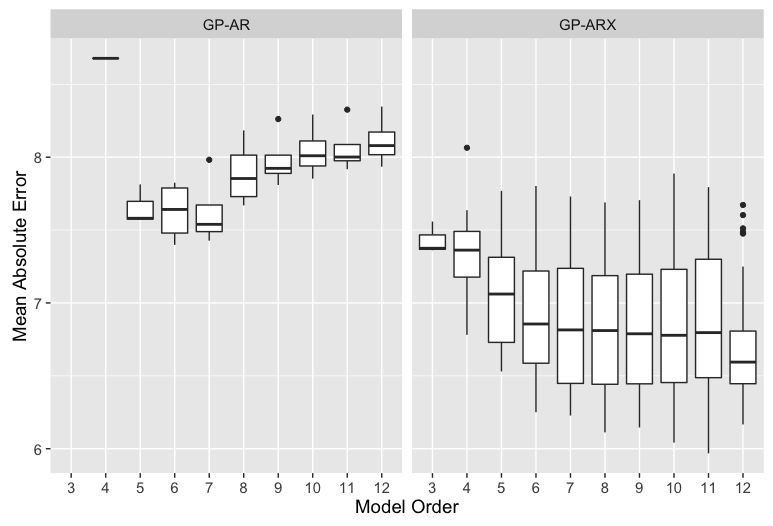
\includegraphics[width=\textwidth]{Compare-mae.png}
\caption{Mean Absolute Error on validation set storms vs model order for GP-AR and GP-ARX. \\ \textbf{Key}: Rectangle borders represent the first and third quartiles, with a horizontal line inside to indicate the median value, outlying points are shown as dots and whiskers indicate the smallest and largest non-outliers}
\label{fig:CompareMae}
\end{figure}

\begin{figure}
\noindent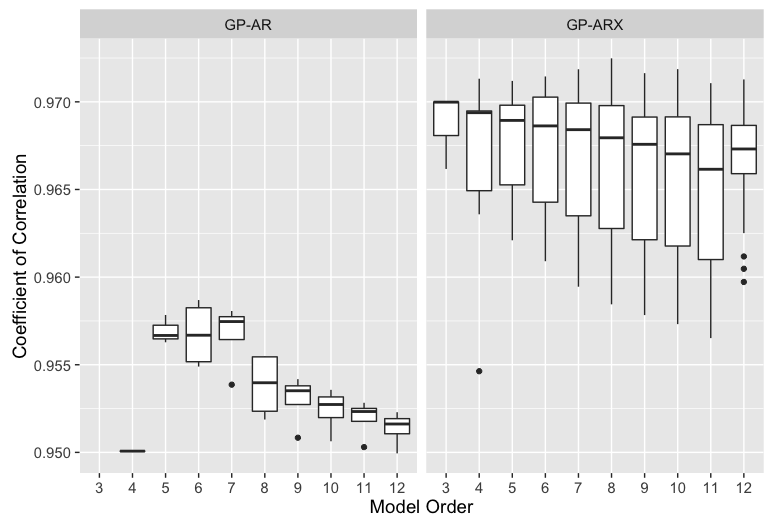
\includegraphics[width=\textwidth]{Compare-cc.png}
\caption{Coefficient of Correlation on validation set storms vs model order for GP-AR and GP-ARX \\ \textbf{Key}: Rectangle borders represent the first and third quartiles, with a horizontal line inside to indicate the median value, outlying points are shown as dots and whiskers indicate the smallest and largest non-outliers}
\label{fig:CompareCC}
\end{figure}


\begin{figure}
\noindent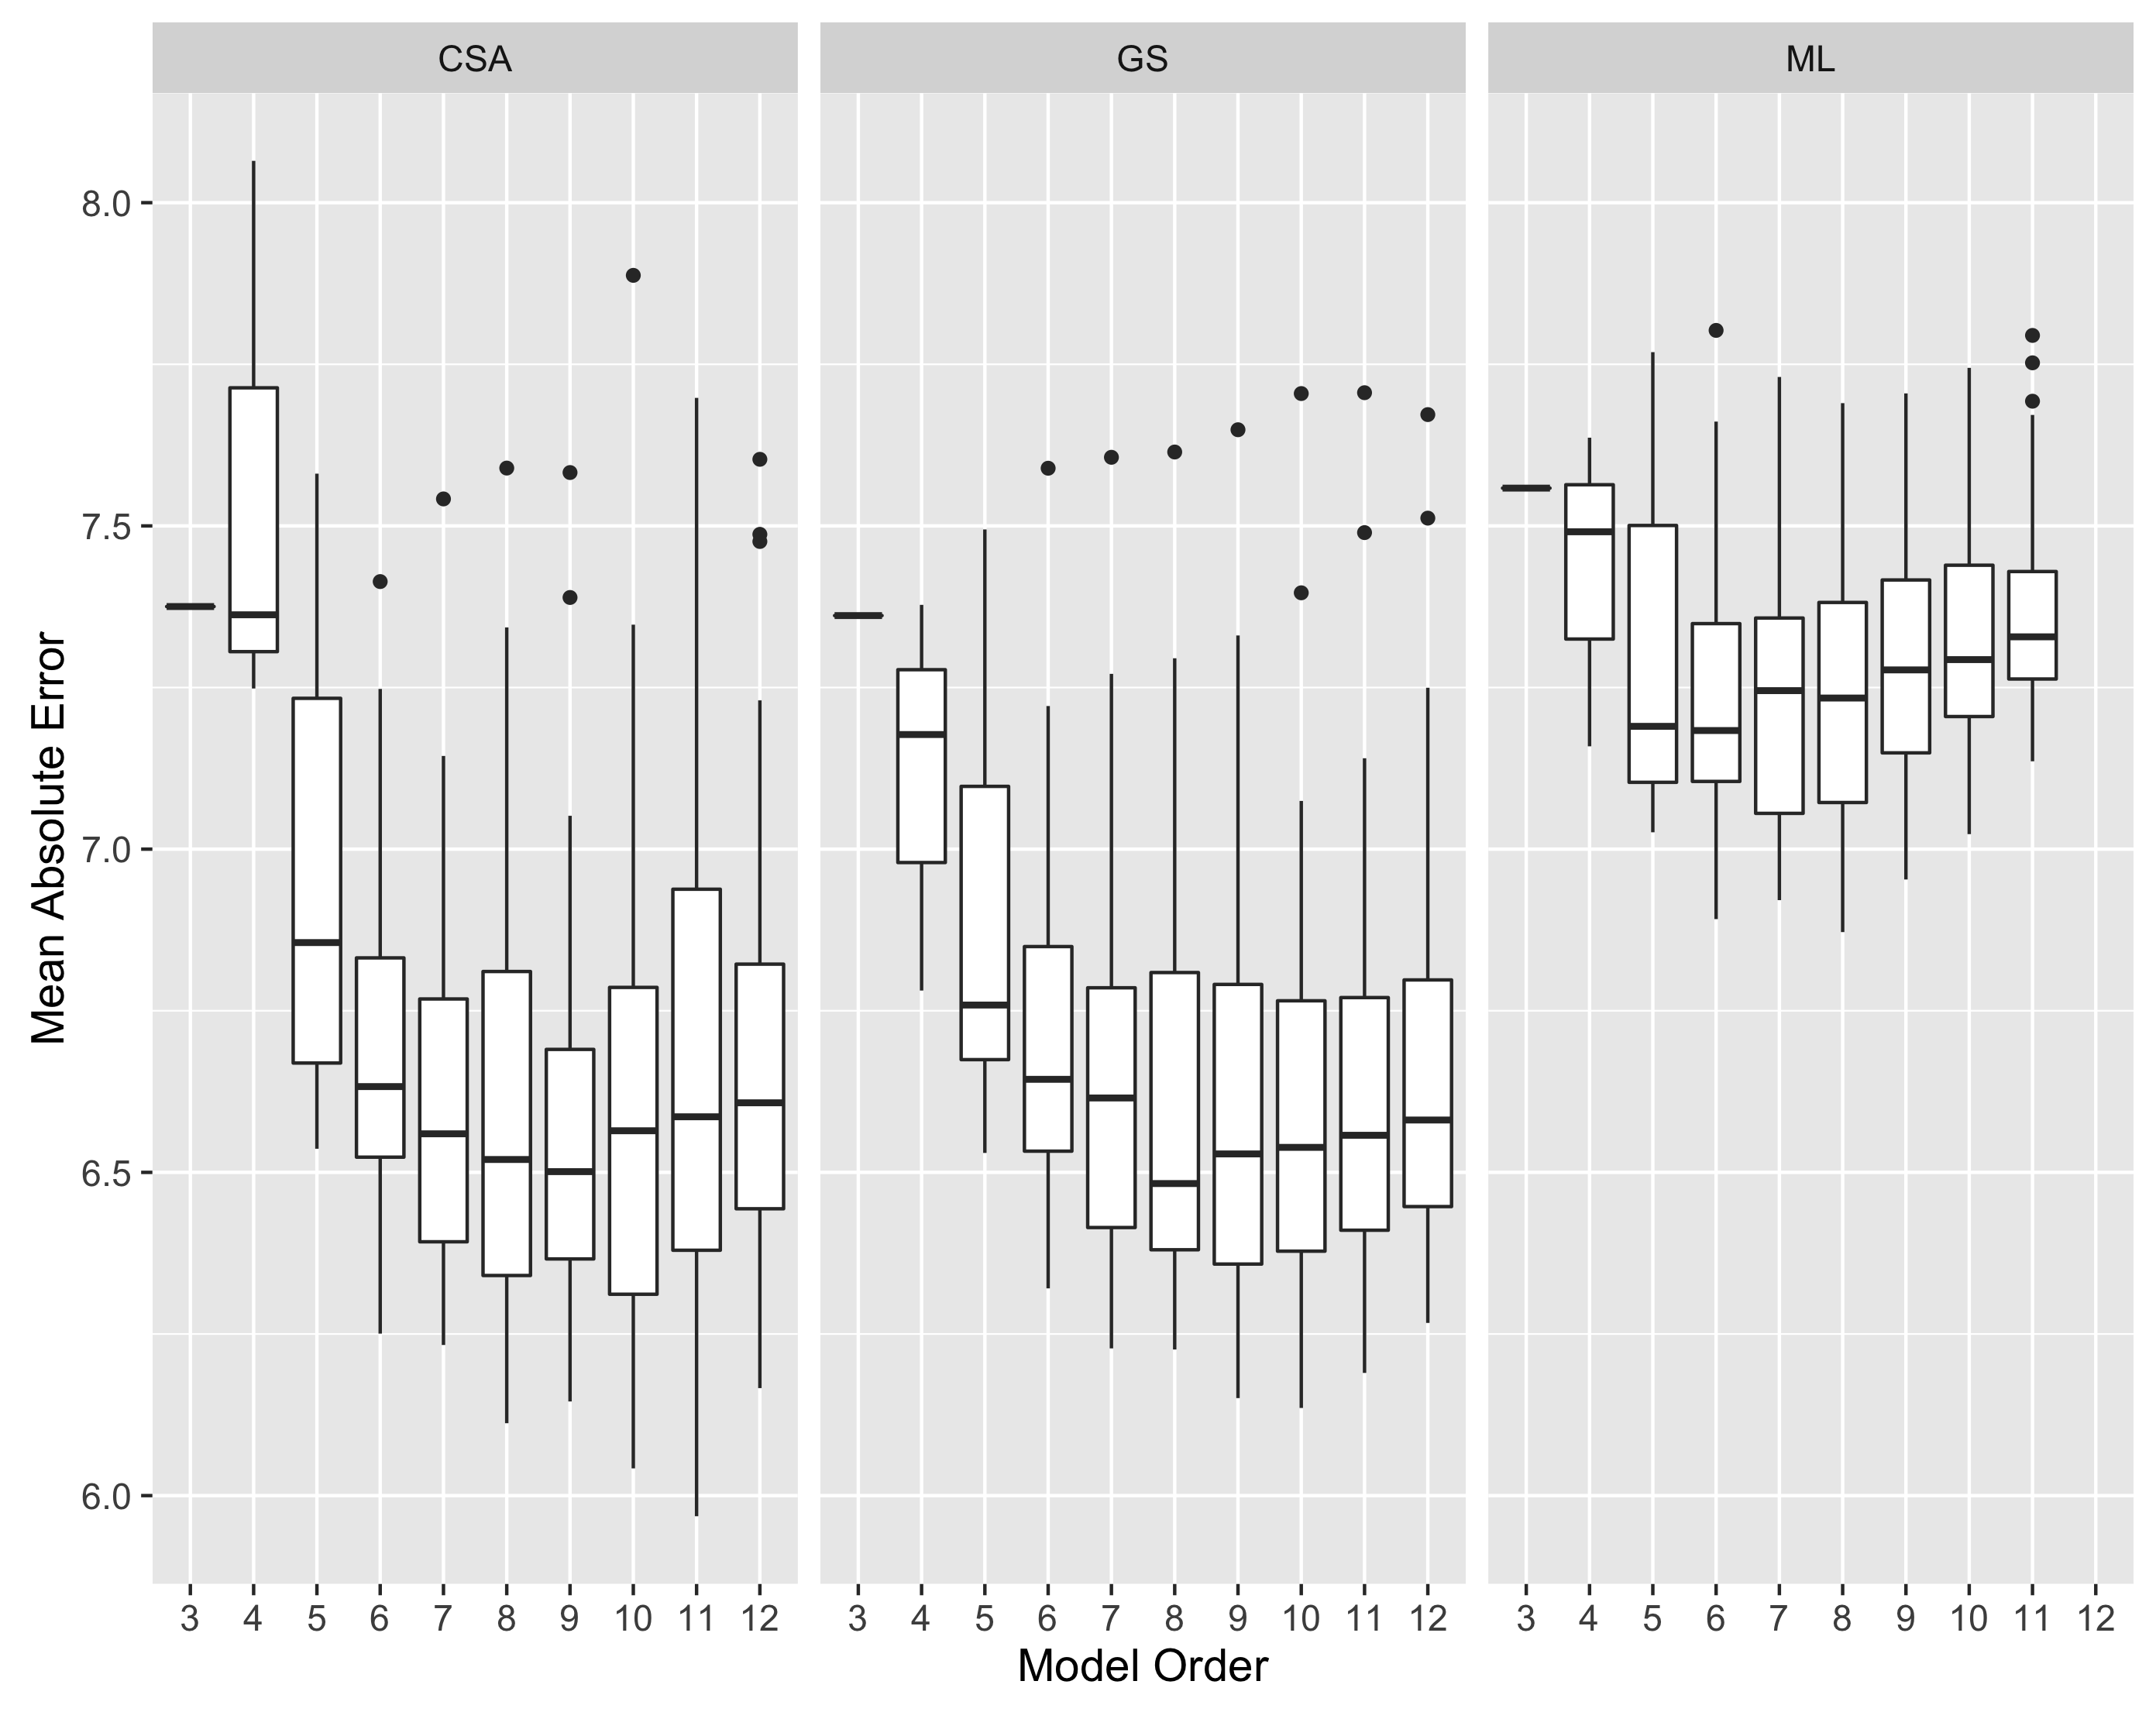
\includegraphics[width=\textwidth]{Compare-mae-arx.png}
\caption{Mean Absolute Error on validation set storms vs model order for GP-AR and GP-ARX for \emph{CSA}, \emph{GS} and \emph{ML} model selection routines \\ \textbf{Key}: Rectangle borders represent the first and third quartiles, with a horizontal line inside to indicate the median value, outlying points are shown as dots and whiskers indicate the smallest and largest non-outliers}
\label{fig:CompareMaeARX}
\end{figure}

\begin{figure}
\noindent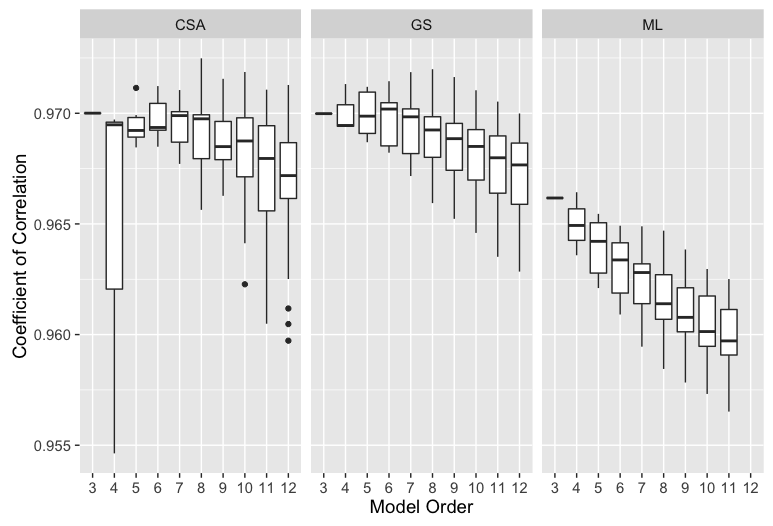
\includegraphics[width=\textwidth]{Compare-cc-arx.png}
\caption{Coefficient of Correlation on validation set storms vs model order for GP-AR and GP-ARX for \emph{CSA}, \emph{GS} and \emph{ML} model selection routines \\ \textbf{Key}: Rectangle borders represent the first and third quartiles, with a horizontal line inside to indicate the median value, outlying points are shown as dots and whiskers indicate the smallest and largest non-outliers}
\label{fig:CompareCCARX}
\end{figure}


\begin{figure}
\noindent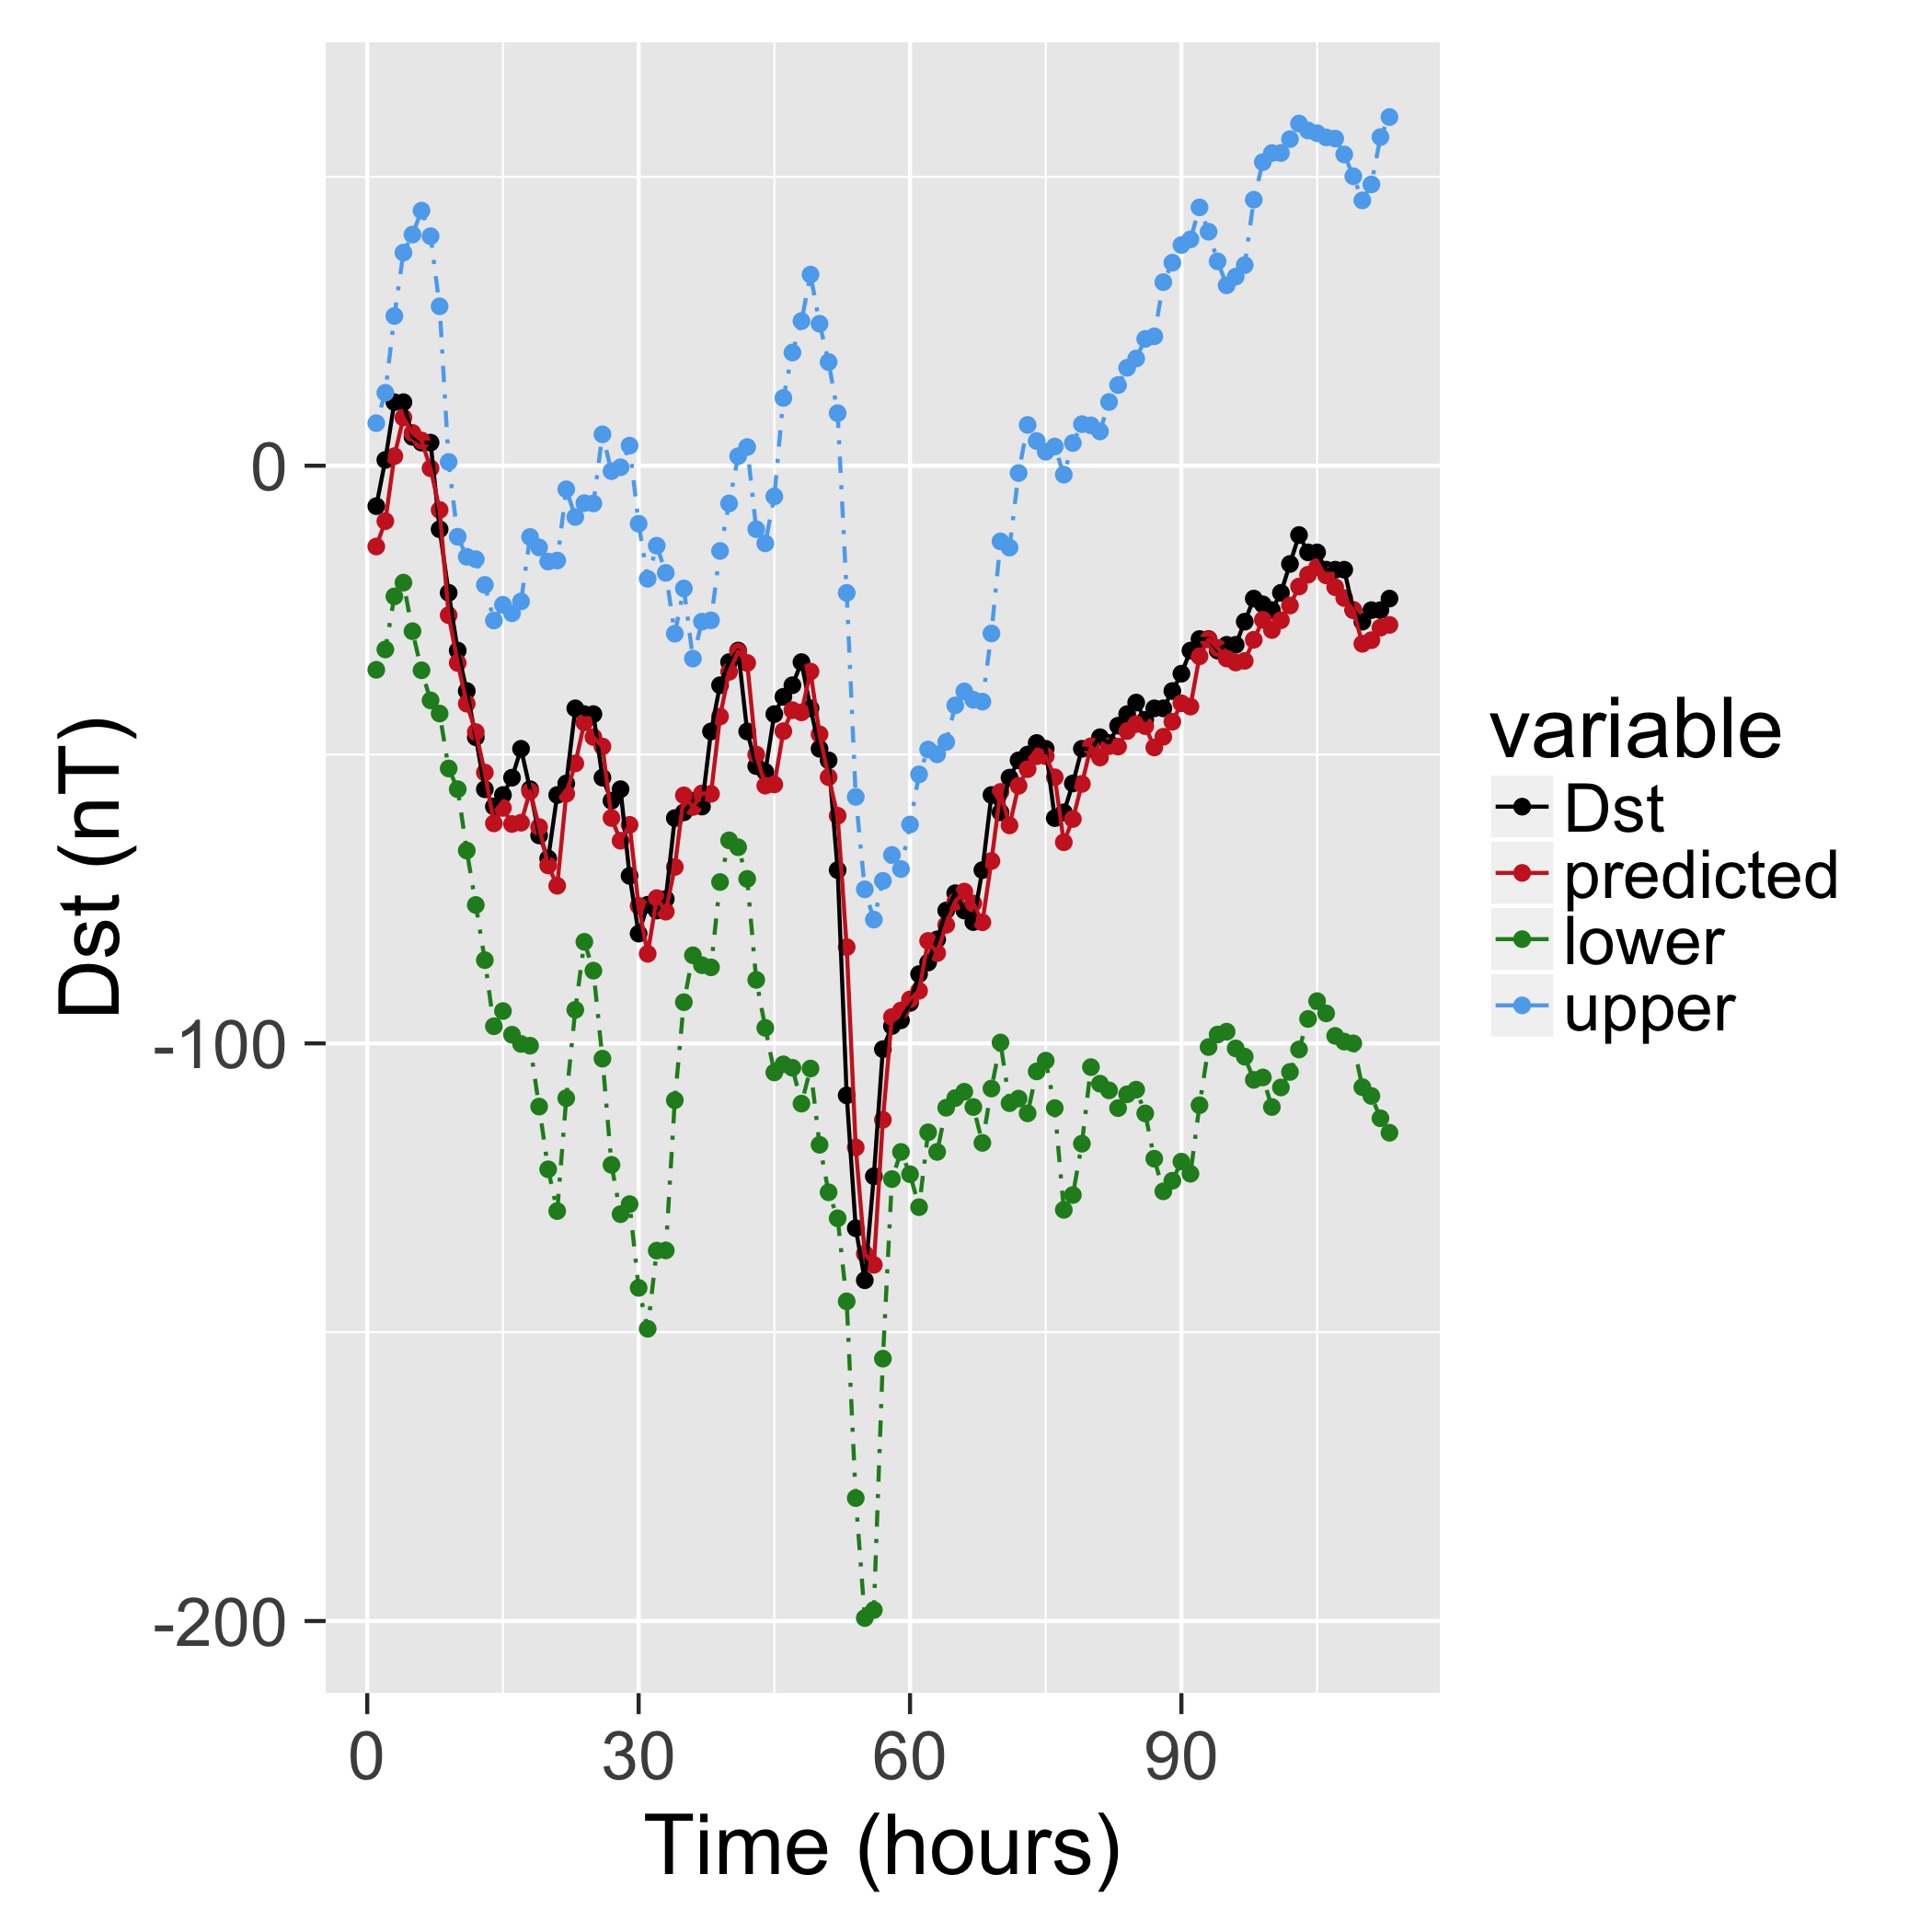
\includegraphics[width=\textwidth]{PredictionsModel1/PredErrBars_Storm43.png}
\caption{OSA Predictions with $\pm \sigma$ error bars for event: 2003/06/17 \DIFdelbeginFL \DIFdelFL{19:00 }\DIFdelendFL to 2003/06/19\DIFdelbeginFL \DIFdelFL{03:00}\DIFdelendFL }
\label{fig:ComparePred1}
\end{figure}


\begin{figure}
\noindent\DIFdelbeginFL %DIFDELCMD < 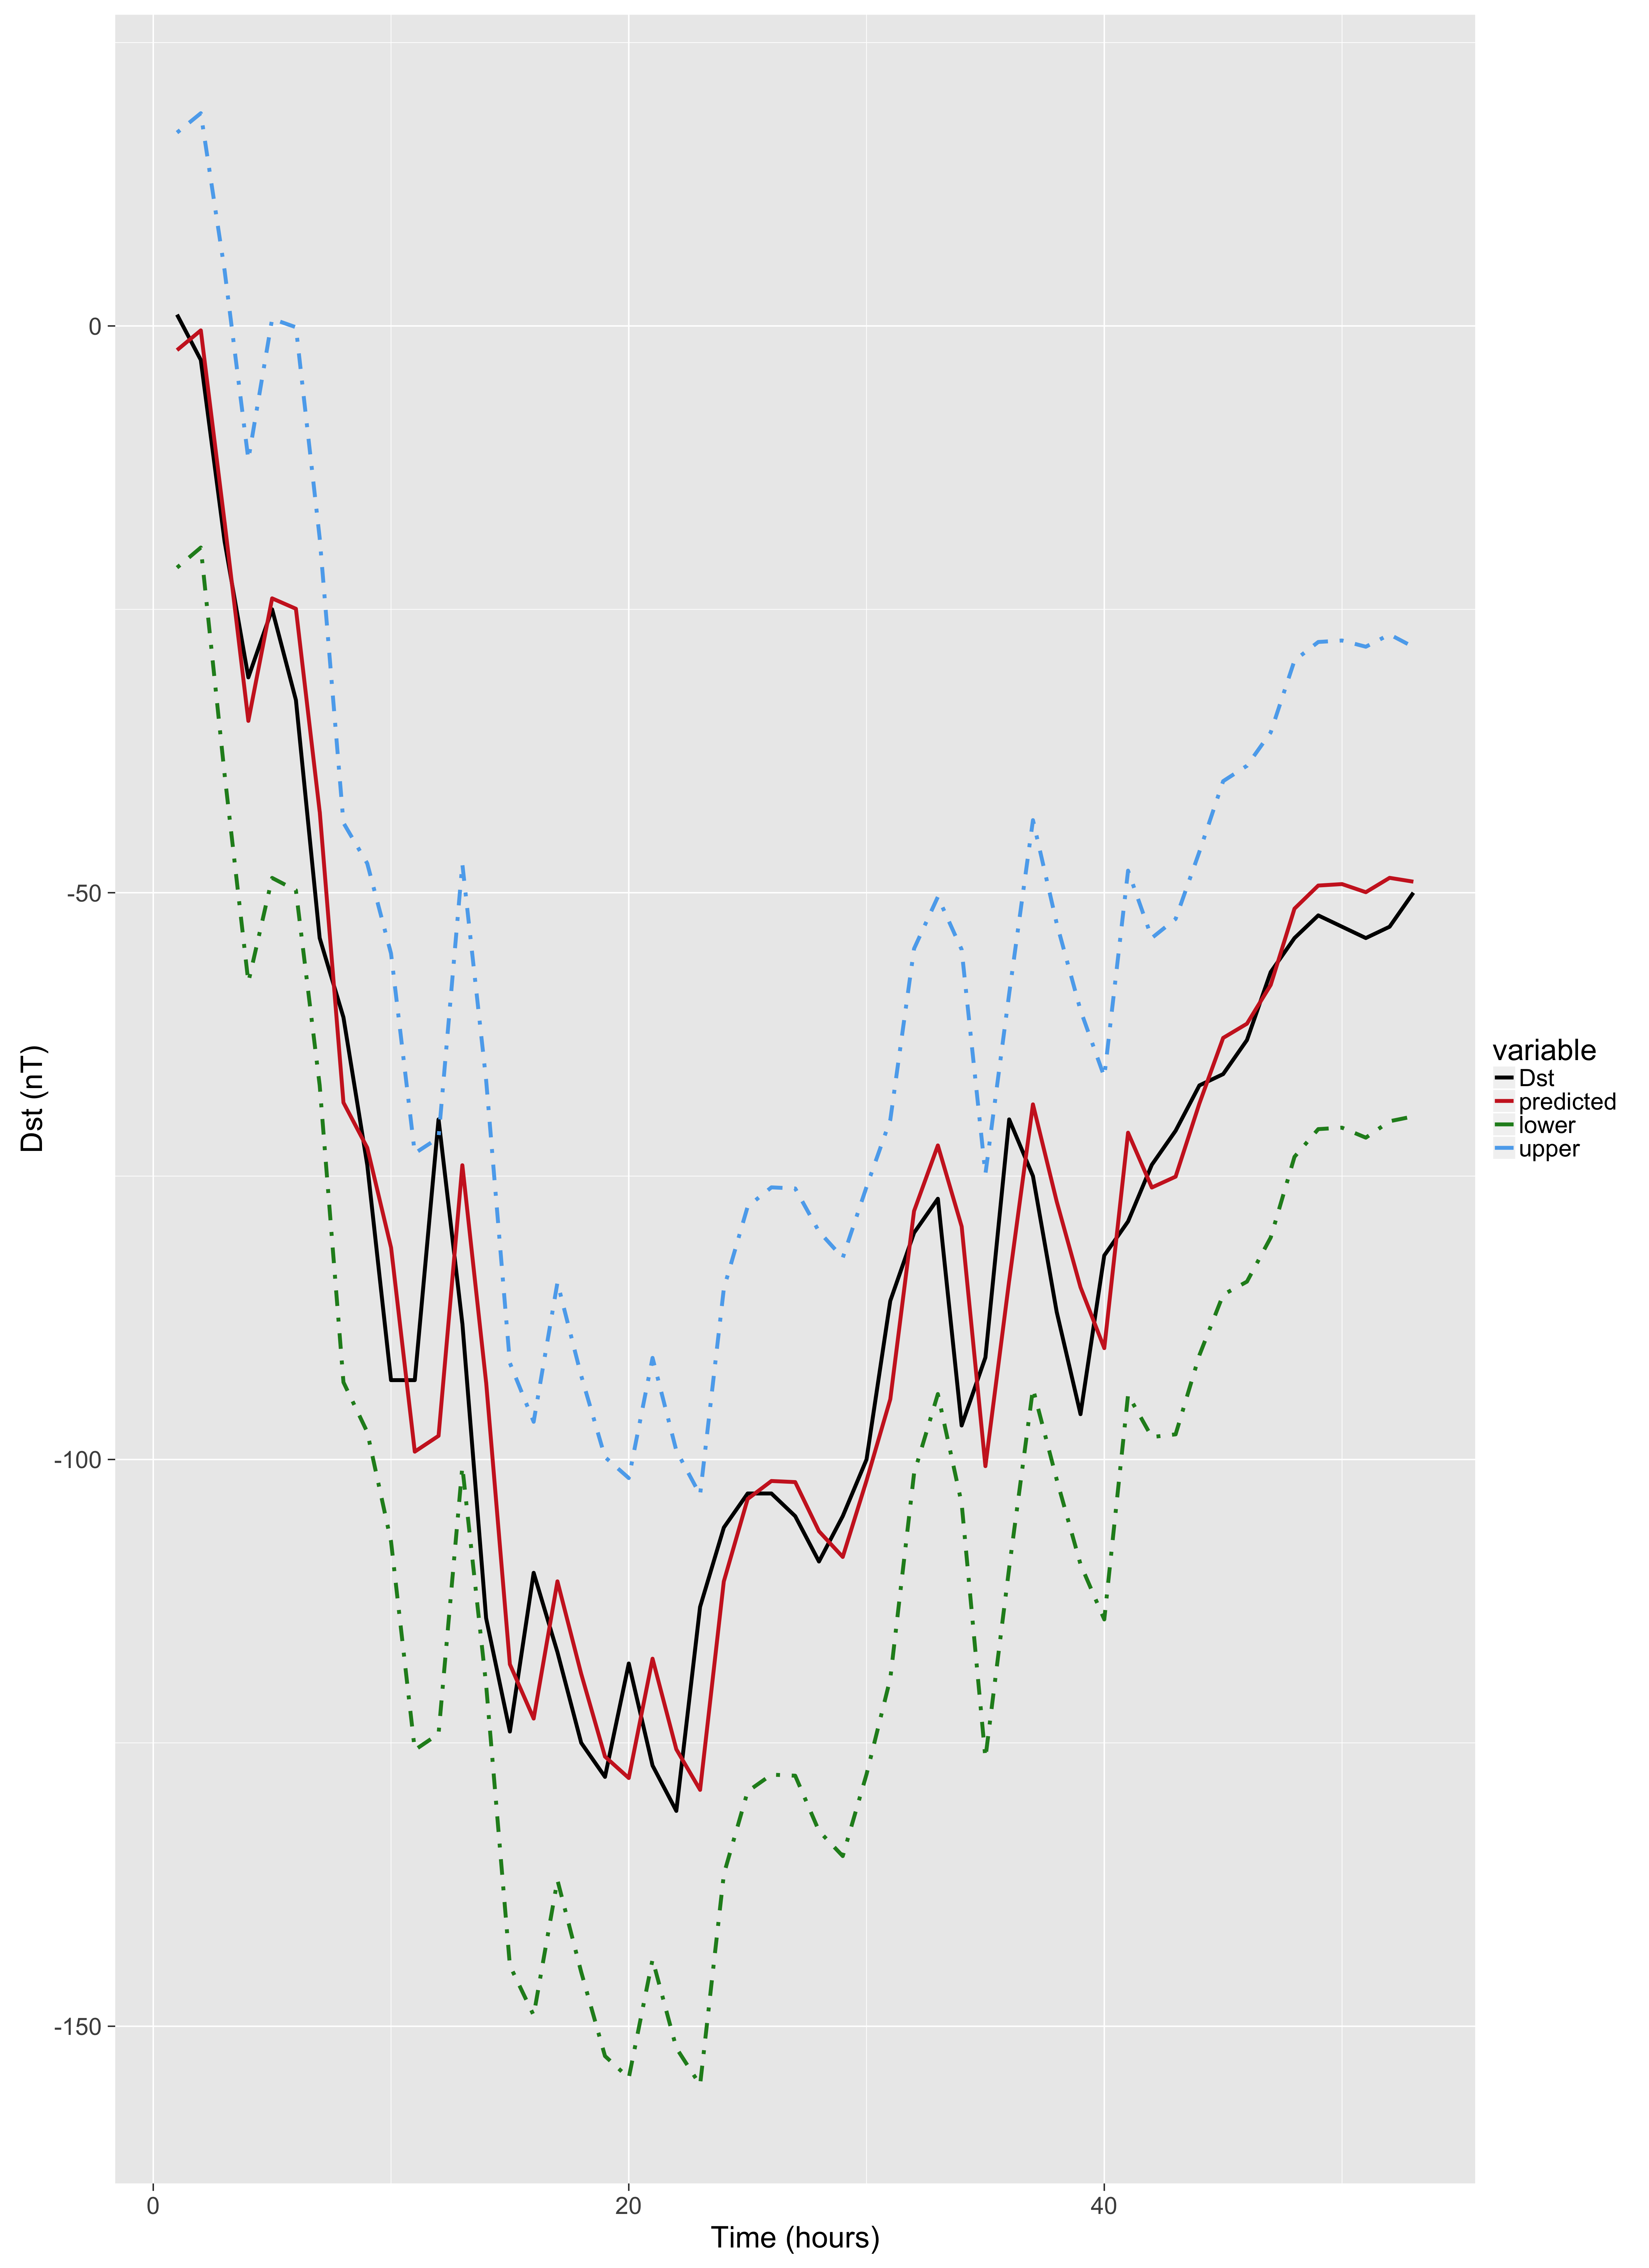
\includegraphics[width=\textwidth]{PredictionsModel1/PredErrBars_Storm8.png}
%DIFDELCMD < %%%
\DIFdelendFL \DIFaddbeginFL 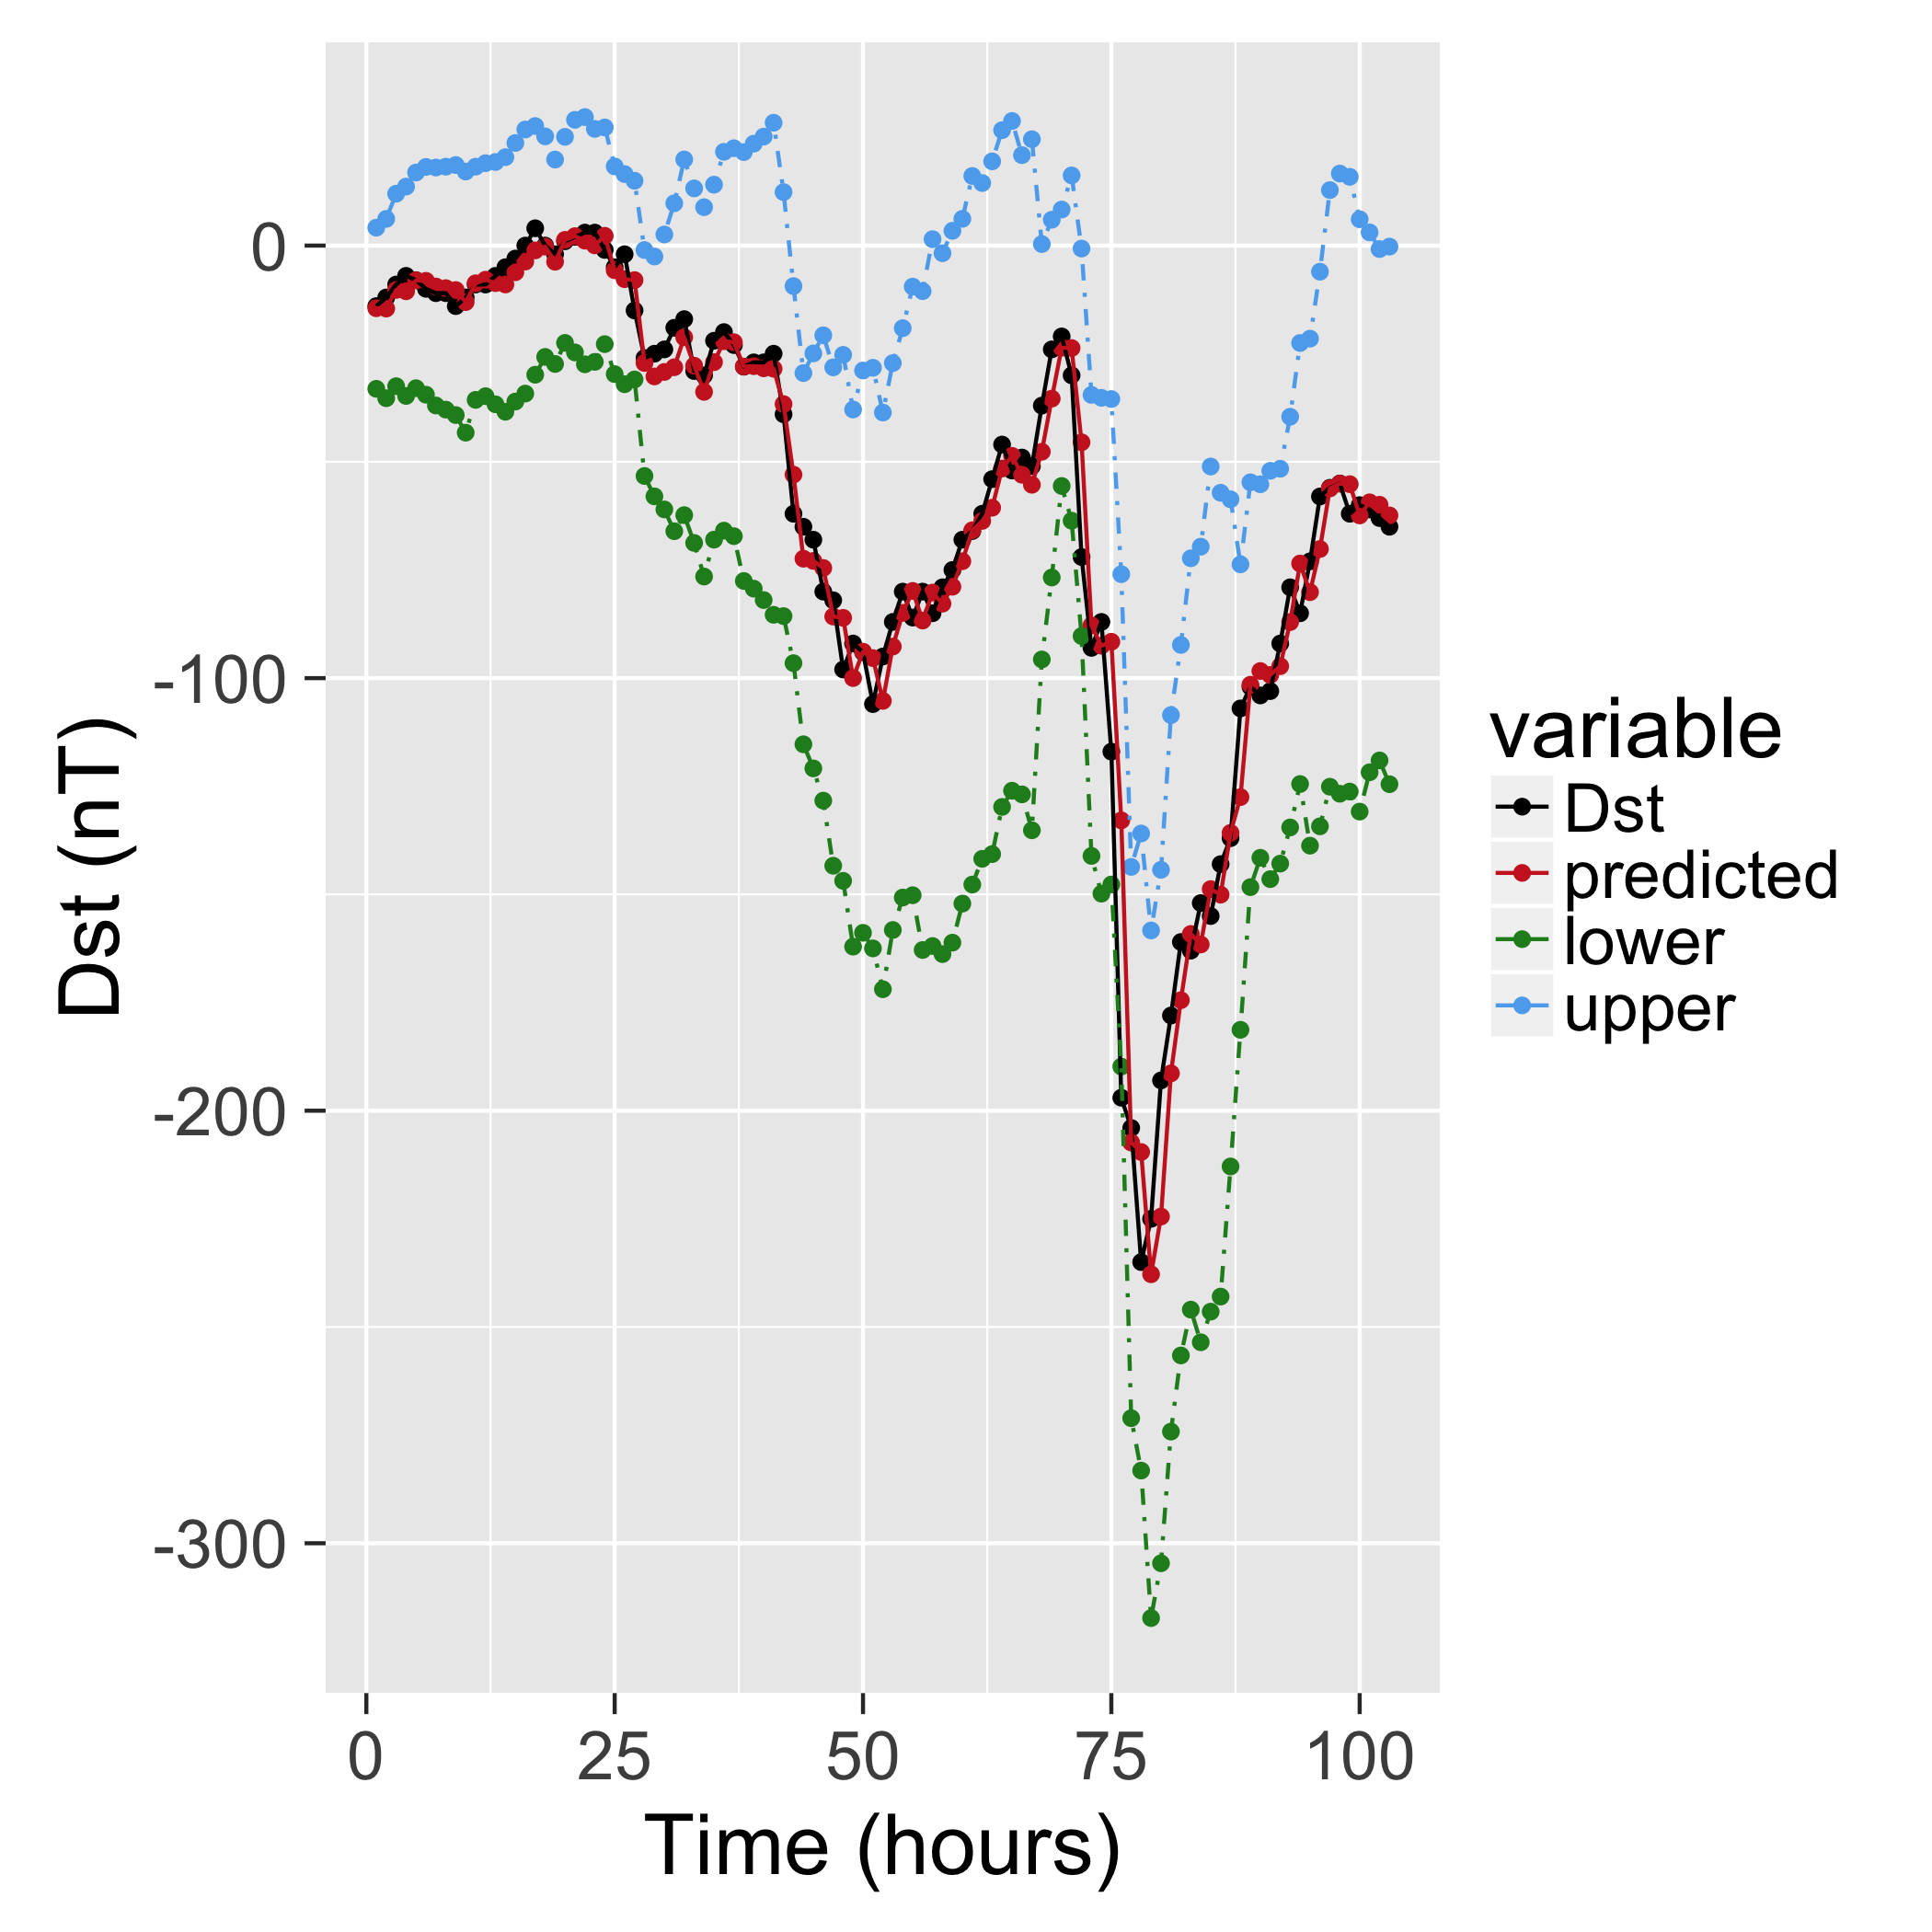
\includegraphics[width=\textwidth]{PredictionsModel1/PredErrBars_Storm16.png}
\DIFaddendFL \caption{OSA Predictions with $\pm \sigma$ error bars for event: \DIFdelbeginFL \DIFdelFL{1998}\DIFdelendFL \DIFaddbeginFL \DIFaddFL{2012}\DIFaddendFL /\DIFdelbeginFL \DIFdelFL{11}\DIFdelendFL \DIFaddbeginFL \DIFaddFL{03}\DIFaddendFL /\DIFdelbeginFL \DIFdelFL{13 00:00 }\DIFdelendFL \DIFaddbeginFL \DIFaddFL{08 }\DIFaddendFL to \DIFdelbeginFL \DIFdelFL{1998}\DIFdelendFL \DIFaddbeginFL \DIFaddFL{2012}\DIFaddendFL /\DIFdelbeginFL \DIFdelFL{11}\DIFdelendFL \DIFaddbeginFL \DIFaddFL{03}\DIFaddendFL /\DIFdelbeginFL \DIFdelFL{15 04:00}\DIFdelendFL \DIFaddbeginFL \DIFaddFL{10}\DIFaddendFL }
\label{fig:ComparePred2}
\end{figure}

\begin{figure}
\noindent\DIFdelbeginFL %DIFDELCMD < 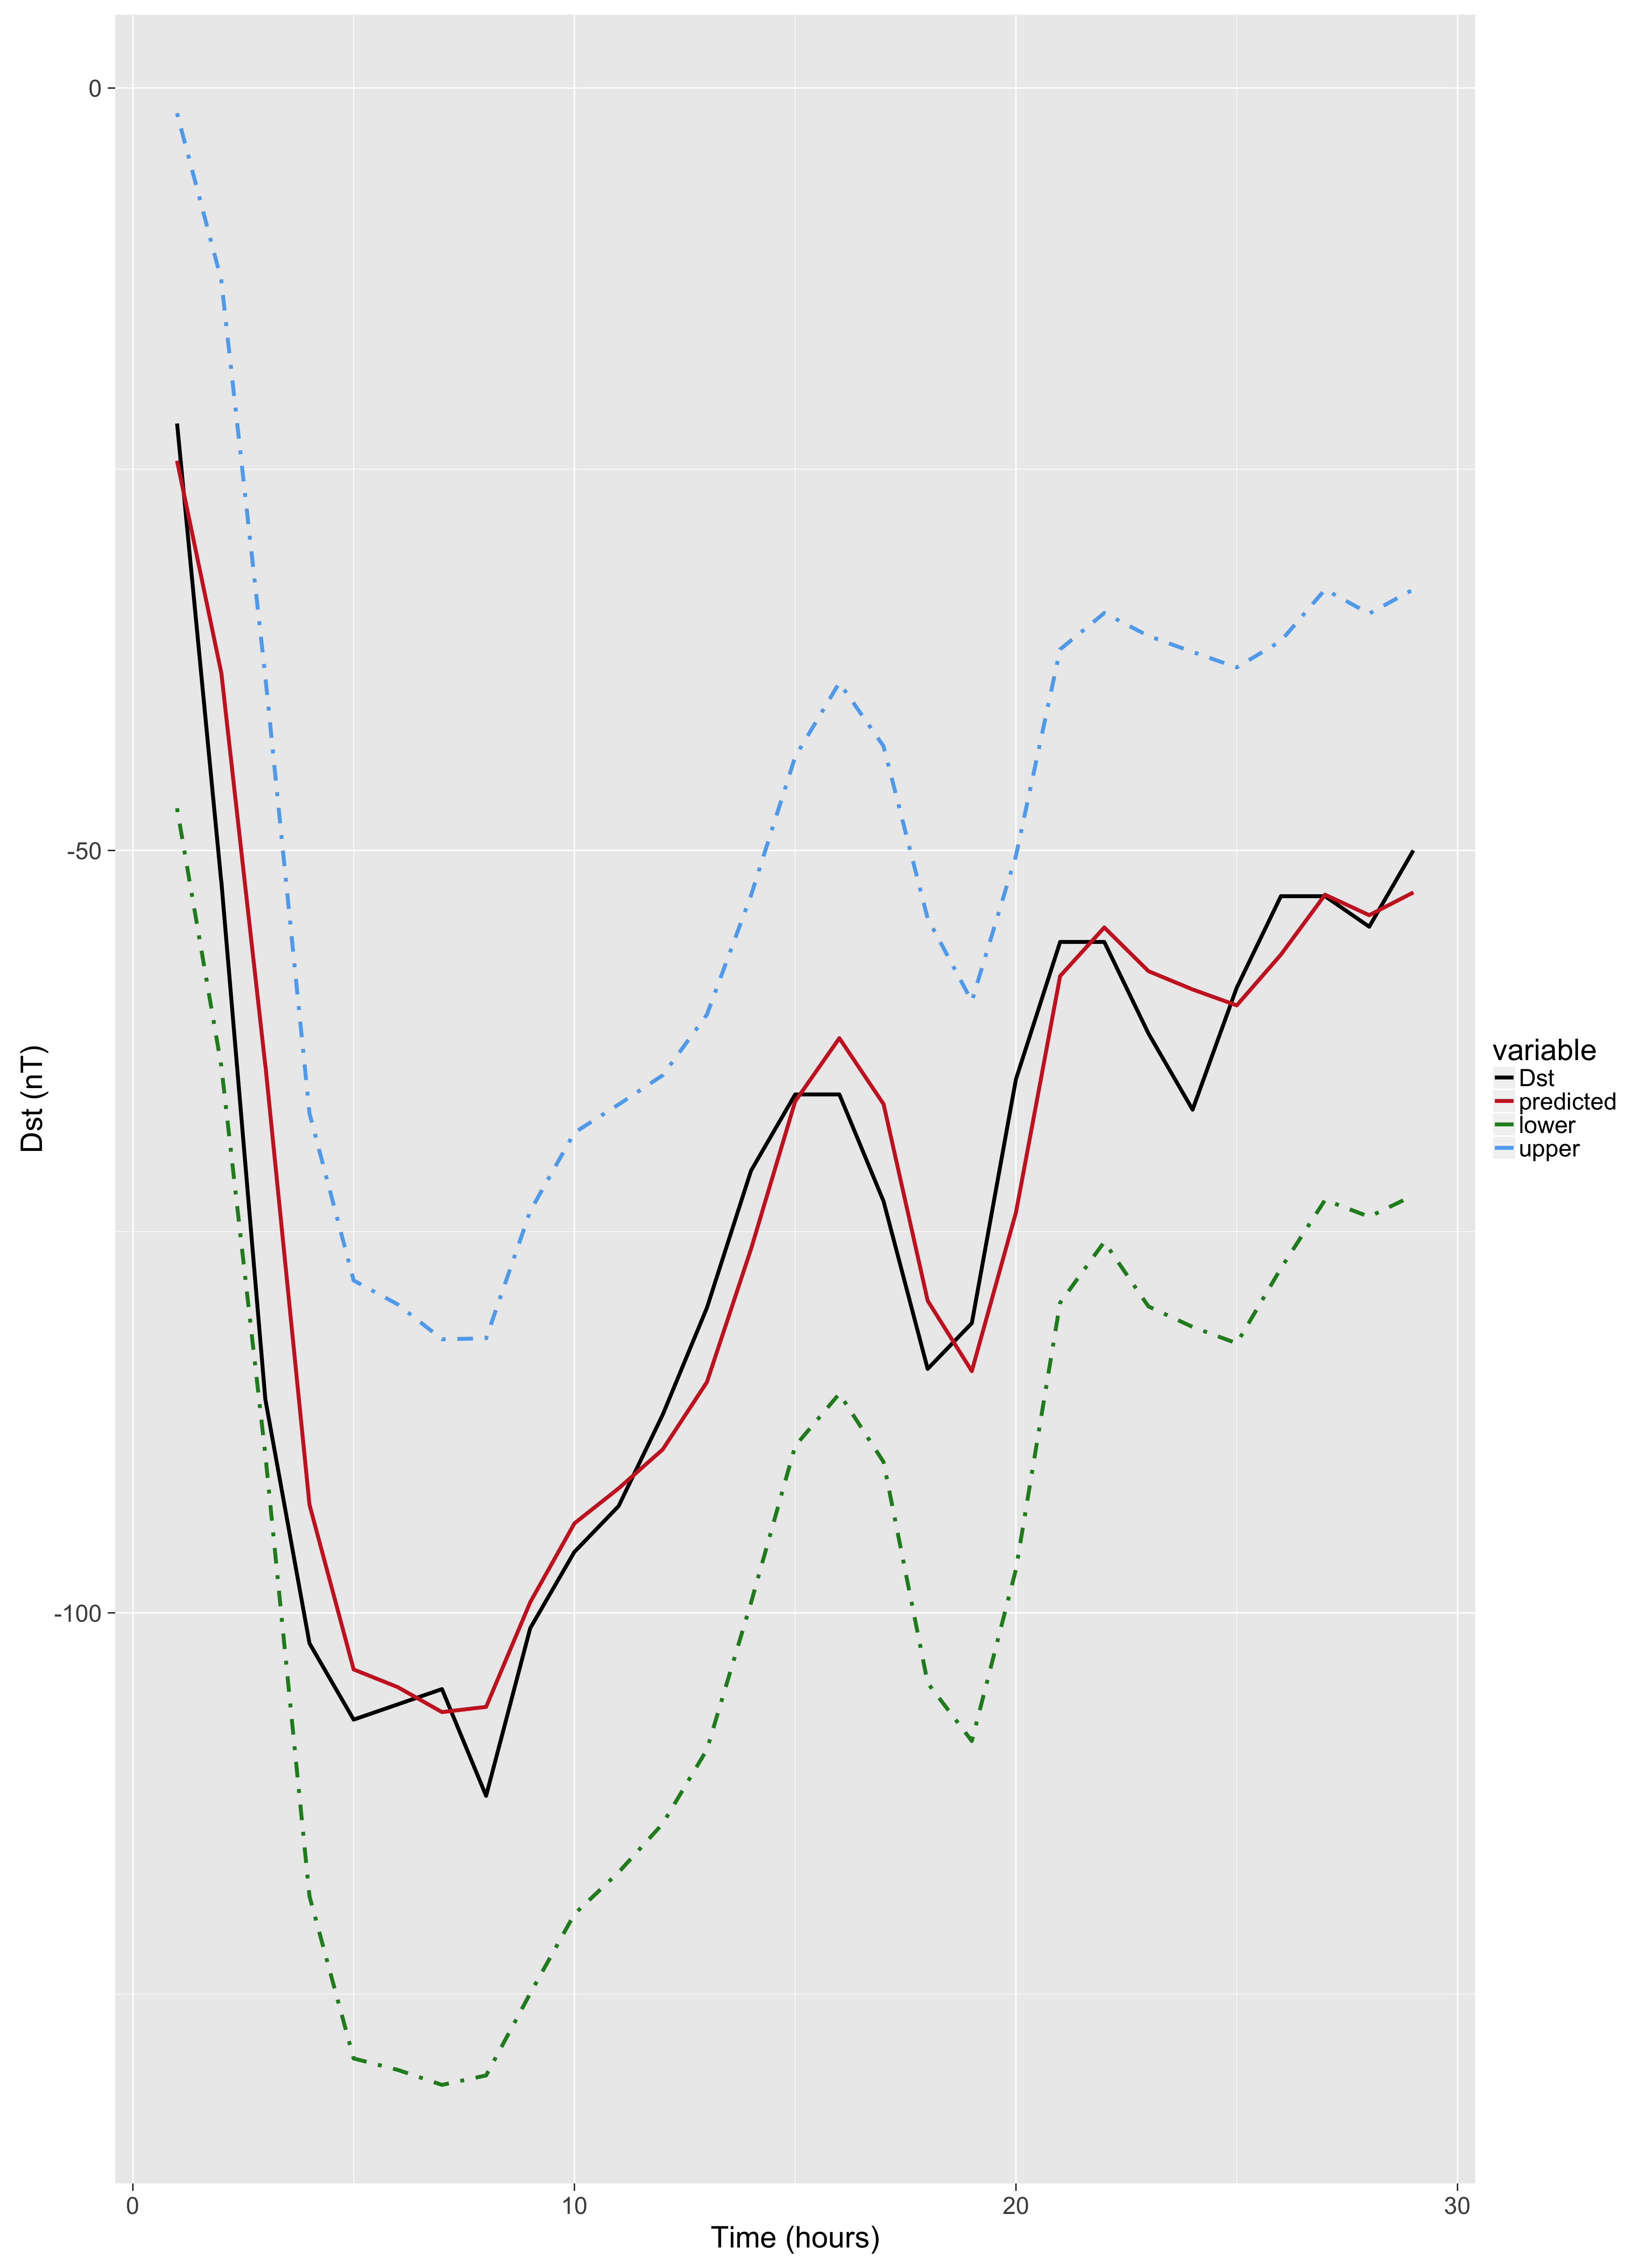
\includegraphics[width=\textwidth]{PredictionsModel1/PredErrBars_Storm9.png}
%DIFDELCMD < %%%
\DIFdelendFL \DIFaddbeginFL 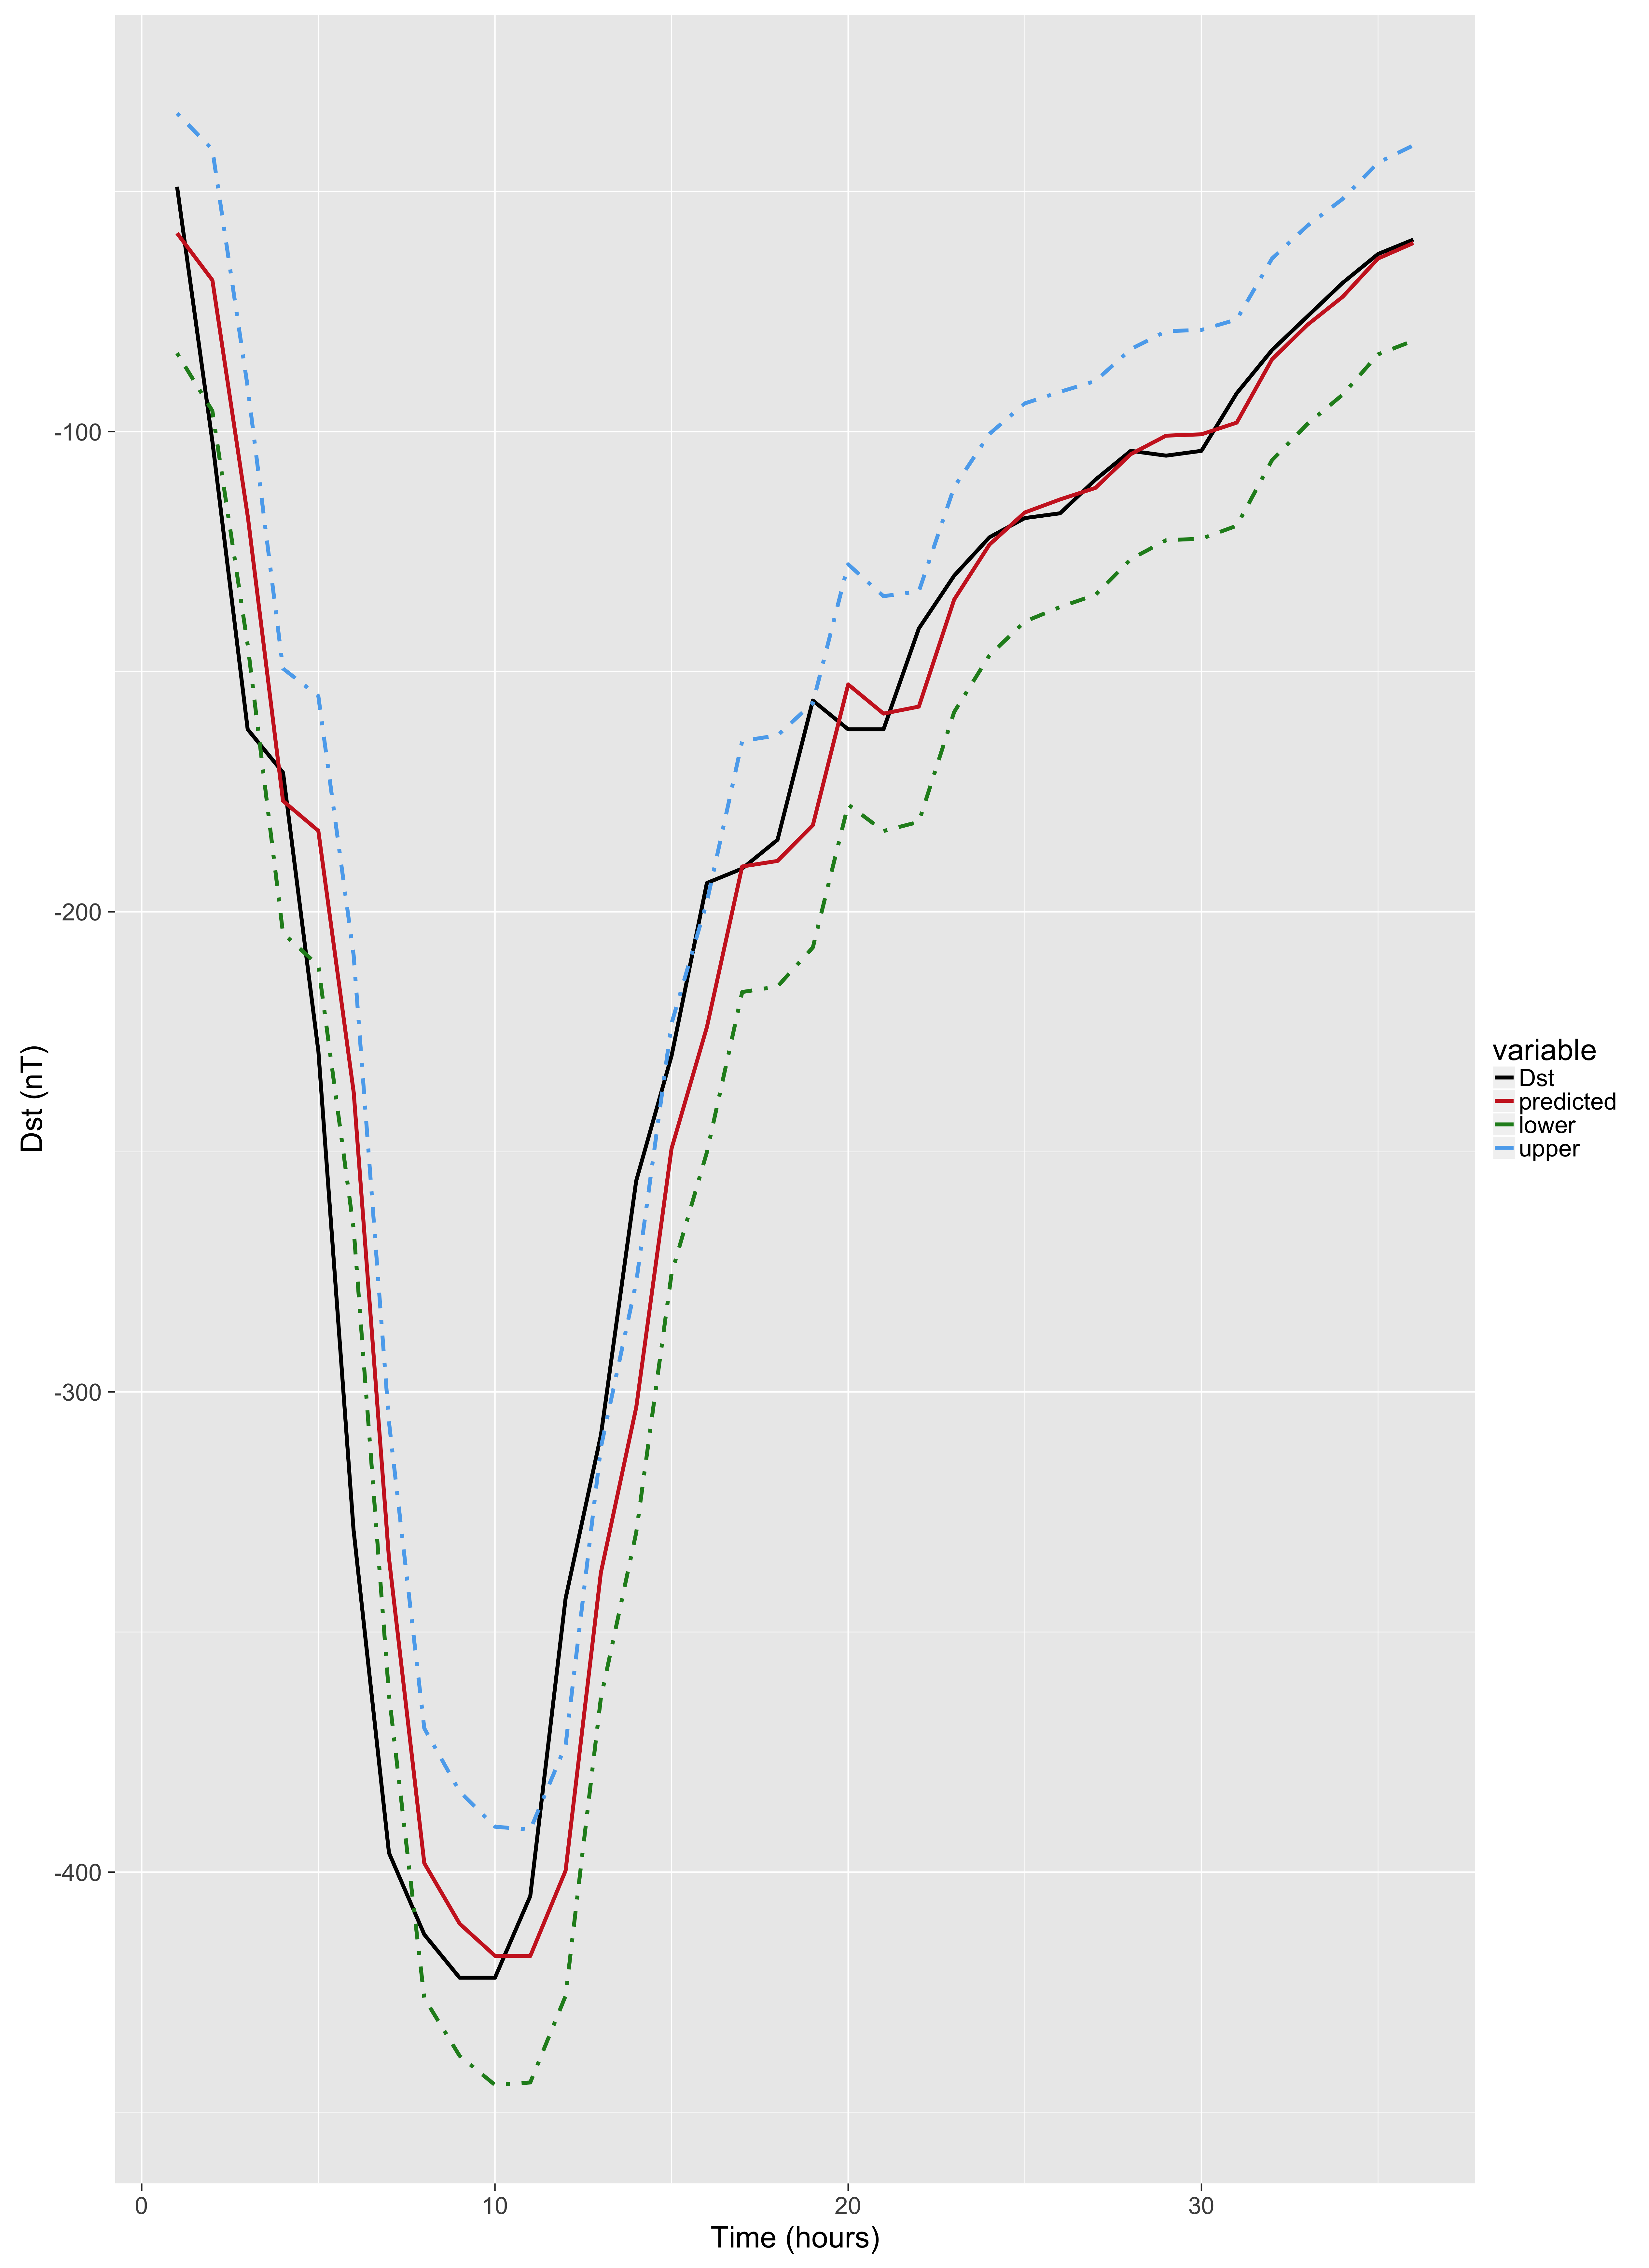
\includegraphics[width=\textwidth]{PredictionsModel1/PredErrBars_Storm46.png}
\DIFaddendFL \caption{OSA Predictions with $\pm \sigma$ error bars for event: \DIFdelbeginFL \DIFdelFL{1999}\DIFdelendFL \DIFaddbeginFL \DIFaddFL{2003}\DIFaddendFL /\DIFdelbeginFL \DIFdelFL{01}\DIFdelendFL \DIFaddbeginFL \DIFaddFL{11}\DIFaddendFL /\DIFdelbeginFL \DIFdelFL{13 16:00 }\DIFdelendFL \DIFaddbeginFL \DIFaddFL{20 }\DIFaddendFL to \DIFdelbeginFL \DIFdelFL{1999}\DIFdelendFL \DIFaddbeginFL \DIFaddFL{2003}\DIFaddendFL /\DIFdelbeginFL \DIFdelFL{01}\DIFdelendFL \DIFaddbeginFL \DIFaddFL{11}\DIFaddendFL /\DIFdelbeginFL \DIFdelFL{14 20:00}\DIFdelendFL \DIFaddbeginFL \DIFaddFL{22}\DIFaddendFL }
\label{fig:ComparePred3}
\end{figure}


%
% ---------------
% EXAMPLE TABLE
%
%\begin{table}
%\caption{Time of the Transition Between Phase 1 and Phase 2\tablenotemark{a}}
%\centering
%\begin{tabular}{l c}
%\hline
% Run  & Time (min)  \\
%\hline
%  $l1$  & 260   \\
%  $l2$  & 300   \\
%  $l3$  & 340   \\
%  $h1$  & 270   \\
%  $h2$  & 250   \\
%  $h3$  & 380   \\
%  $r1$  & 370   \\
%  $r2$  & 390   \\
%\hline
%\end{tabular}
%\tablenotetext{a}{Footnote text here.}
%\end{table}

\begin{table}[h]
\caption{Popular Kernel functions used in GPR models}
\centering
\begin{tabular}{l c c}
\hline
 Name  & Expression & Hyperparameters  \\
\hline
  Radial Basis Function (RBF)  & $\frac{1}{2} exp(-||\mathbf{x} - \mathbf{y}||^2/l^2)$  & $l \in \mathbb{R}$   \\

  Polynomial  & $(\mathbf{x}^\intercal \mathbf{y} + b)^d$ & $b \in \mathbb{R}, d \in \mathbb{N}$   \\

  Laplacian  & $exp(-||\mathbf{x} - \mathbf{y}||_{1}/\theta)$  & $\theta \in \mathbb{R}^+$  \\

  Student's T  & $1/(1 + ||\mathbf{x} - \mathbf{y}||_{2}^d)$ & $d \in \mathbb{R}^{+}$\\

  Maximum Likelihood Perceptron  & $sin^{-1}(\frac{w\mathbf{x}^\intercal \mathbf{y} + b}{\sqrt{w\mathbf{x}^\intercal \mathbf{x} + b + 1} \sqrt{w\mathbf{y}^\intercal \mathbf{y} + b + 1}})$ & $w, b \in \mathbb{R}^{+}$\\
\hline
\end{tabular}
\label{table:kernel}
\end{table}

\begin{table}[h]
\centering
\caption{Settings of model selection procedures}
\begin{tabular}{l c c c}
\hline
Procedure & Grid Size & Step & Max Iterations \\
\hline
Grid Search & 10 & 0.2 & NA \\
Coupled Simulated Annealing & 4 & 0.2 & 30 \\
Maximum likelihood & NA & 0.2 & 150\\
\end{tabular}
\label{table:modelselection}
\end{table}


\begin{table}[h]
\centering
\caption{Evaluation results for models on storm events listed in table \ref{table:teststorms}}
\label{table:results}
\begin{tabular}{l c c c}
\hline
Model & Mean Absolute Error & Root Mean Square Error & Coefficient of Correlation\\ \hline
GP-ARX & \DIFdelbeginFL \DIFdelFL{7.252 }\DIFdelendFL \DIFaddbeginFL \DIFaddFL{7.219 }\DIFaddendFL & \DIFdelbeginFL \DIFdelFL{11.93 }\DIFdelendFL \DIFaddbeginFL \DIFaddFL{11.88 }\DIFaddendFL & 0.972\\
GP-AR & 8.37 & 14.04 & 0.963\\
Persistence & 9.182 & 14.94 & 0.957\\
\end{tabular}
\end{table}

\begin{table}[h]
\centering
\caption{Storm events used for model selection of GP-AR and GP-ARX}
\label{table:validationstorms}
\begin{tabular}{llllll}
\hline
Event Id & Start Date & Start Hour & End Date & End Hour & min. Dst \\ \hline
1 & 1995/03/26 & 0500 & 1995/03/26 & 2300 & −107 \\
2 & 1995/04/07 & 1300 & 1995/04/09 & 0900 & −149 \\
3 & 1995/09/27 & 0100 & 1995/09/28 & 0400 & −108 \\
4 & 1995/10/18 & 1300 & 1995/10/19 & 1400 & −127 \\
5 & 1996/10/22 & 2200 & 1996/10/23 & 1100 & −105 \\
6 & 1997/04/21 & 1000 & 1997/04/22 & 0900 & −107 \\
7 & 1997/05/15 & 0300 & 1997/05/16 & 0000 & −115 \\
8 & 1997/10/10 & 1800 & 1997/10/11 & 1900 & −130 \\
9 & 1997/11/07 & 0000 & 1997/11/07 & 1800 & −110 \\
10 & 1997/11/22 & 2100 & 1997/11/24 & 0400 & −108 \\
11 & 2005/06/12 & 1700 & 2005/06/13 & 1900 & −106 \\
12 & 2005/08/31 & 1200 & 2005/09/01 & 1200 & −122 \\
13 & 2006/12/14 & 2100 & 2006/12/16 & 0300 & −162 \\
14 & 2011/09/26 & 1400 & 2011/09/27 & 1200 & −101 \\
15 & 2011/10/24 & 2000 & 2011/10/25 & 1400 & −132 \\
16 & 2012/03/08 & 1200 & 2012/03/10 & 1600 & −131 \\
17 & 2012/04/23 & 1100 & 2012/04/24 & 1300 & −108 \\
18 & 2012/07/15 & 0100 & 2012/07/16 & 2300 & −127 \\
19 & 2012/09/30 & 1300 & 2012/10/01 & 1800 & −119 \\
20 & 2012/10/08 & 0200 & 2012/10/09 & 1700 & −105 \\
21 & 2012/11/13 & 1800 & 2012/11/14 & 1800 & −108 \\
22 & 2013/03/17 & 0700 & 2013/03/18 & 1000 & −132 \\
23 & 2013/05/31 & 1800 & 2013/06/01 & 2000 & −119 \\
24 & 2014/02/18 & 1500 & 2014/02/19 & 1600 & −112
\end{tabular}
\end{table}


\begin{table}[h]
\fontsize{9}{10.4}\selectfont
\centering
\caption{Storm events used to evaluate GP-AR and GP-ARX models}
\label{table:teststorms}
\begin{tabular}{cccccc}
\hline
Event Id & Start Date & Start Time & End Date & End Time & min. Dst \\ \hline
1 & 1998/02/17 & 1200 & 1998/02/18 & 1000 & -100 \\
2 & 1998/03/10 & 1100 & 1998/03/11 & 1800 & -116 \\
3 & 1998/05/04 & 0200 & 1998/05/05 & 0200 & -205 \\
4 & 1998/08/26 & 1000 & 1998/08/29 & 0700 & -155 \\
5 & 1998/09/25 & 0100 & 1998/09/26 & 0000 & -207 \\
6 & 1998/10/19 & 0500 & 1998/10/20 & 0800 & -112 \\
7 & 1998/11/09 & 0300 & 1998/11/10 & 1600 & -142 \\
8 & 1998/11/13 & 0000 & 1998/11/15 & 0400 & -131 \\
9 & 1999/01/13 & 1600 & 1999/01/14 & 2000 & -112 \\
10 & 1999/02/18 & 0300 & 1999/02/19 & 2100 & -123 \\
11 & 1999/09/22 & 2000 & 1999/09/23 & 2300 & -173 \\
12 & 1999/10/22 & 0000 & 1999/10/23 & 1400 & -237 \\
13 & 2000/02/12 & 0500 & 2000/02/13 & 1500 & -133 \\
14 & 2000/04/06 & 1700 & 2000/04/08 & 0900 & -288 \\
15 & 2000/05/24 & 0100 & 2000/05/25 & 2000 & -147 \\
16 & 2000/08/10 & 2000 & 2000/08/11 & 1800 & \DIFdelbeginFL \DIFdelFL{-106 }\DIFdelendFL \DIFaddbeginFL \DIFaddFL{-230 }\DIFaddendFL \\
17 & 2000/08/12 & 0200 & 2000/08/13 & 1700 & -235 \\
18 & 2000/10/13 & 0200 & 2000/10/14 & 2300 & -107 \\
19 & 2000/10/28 & 2000 & 2000/10/29 & 2000 & -127 \\
20 & 2000/11/06 & 1300 & 2000/11/07 & 1800 & -159 \\
21 & 2000/11/28 & 1800 & 2000/11/29 & 2300 & -119 \\
22 & 2001/03/19 & 1500 & 2001/03/21 & 2300 & -149 \\
23 & 2001/03/31 & 0400 & 2001/04/01 & 2100 & -387 \\
24 & 2001/04/11 & 1600 & 2001/04/13 & 0700 & -271 \\
25 & 2001/04/18 & 0100 & 2001/04/18 & 1300 & -114 \\
26 & 2001/04/22 & 0200 & 2001/04/23 & 1500 & -102 \\
27 & 2001/08/17 & 1600 & 2001/08/18 & 1600 & -105 \\
28 & 2001/09/30 & 2300 & 2001/10/02 & 0000 & -148 \\
29 & 2001/10/21 & 1700 & 2001/10/24 & 1100 & -187 \\
30 & 2001/10/28 & 0300 & 2001/10/29 & 2200 & -157 \\
31 & 2002/03/23 & 1400 & 2002/03/25 & 0500 & -100 \\
32 & 2002/04/17 & 1100 & 2002/04/19 & 0200 & -127 \\
33 & 2002/04/19 & 0900 & 2002/04/21 & 0600 & -149 \\
34 & 2002/05/11 & 1000 & 2002/05/12 & 1600 & -110 \\
35 & 2002/05/23 & 1200 & 2002/05/24 & 2300 & -109 \\
36 & 2002/08/01 & 2300 & 2002/08/02 & 0900 & -102 \\
37 & 2002/09/04 & 0100 & 2002/09/05 & 0000 & -109 \\
38 & 2002/09/07 & 1400 & 2002/09/08 & 2000 & -181 \\
39 & 2002/10/01 & 0600 & 2002/10/03 & 0800 & -176 \\
40 & 2002/10/03 & 1000 & 2002/10/04 & 1800 & -146 \\
41 & 2002/11/20 & 1600 & 2002/11/22 & 0600 & -128 \\
42 & 2003/05/29 & 2000 & 2003/05/30 & 1000 & -144 \\
43 & 2003/06/17 & 1900 & 2003/06/19 & 0300 & -141 \\
44 & 2003/07/11 & 1500 & 2003/07/12 & 1600 & -105 \\
45 & 2003/08/17 & 1800 & 2003/08/19 & 1100 & -148 \\
46 & 2003/11/20 & 1200 & 2003/11/22 & 0000 & -422 \\
47 & 2004/01/22 & 0300 & 2004/01/24 & 0000 & -149 \\
48 & 2004/02/11 & 1000 & 2004/02/12 & 0000 & -105 \\
49 & 2004/04/03 & 1400 & 2004/04/04 & 0800 & -112 \\
50 & 2004/07/22 & 2000 & 2004/07/23 & 2000 & -101 \\
51 & 2004/07/24 & 2100 & 2004/07/26 & 1700 & -148 \\
52 & 2004/07/26 & 2200 & 2004/07/30 & 0500 & -197 \\
53 & 2004/08/30 & 0500 & 2004/08/31 & 2100 & -126 \\
54 & 2004/11/07 & 2100 & 2004/11/08 & 2100 & -373 \\
55 & 2004/11/09 & 1100 & 2004/11/11 & 0900 & -289 \\
56 & 2004/11/11 & 2200 & 2004/11/13 & 1300 & -109 \\
57 & 2005/01/21 & 1800 & 2005/01/23 & 0500 & -105 \\
58 & 2005/05/07 & 2000 & 2005/05/09 & 1000 & -127 \\
59 & 2005/05/29 & 2200 & 2005/05/31 & 0800 & -138 \\
60 & 2005/06/12 & 1700 & 2005/06/13 & 1900 & -106 \\
61 & 2005/08/31 & 1200 & 2005/09/01 & 1200 & -131 \\
62 & 2006/04/13 & 2000 & 2006/04/14 & 2300 & -111 \\
63 & 2006/12/14 & 2100 & 2006/12/16 & 0300 & -147 \\ \hline
\end{tabular}%
\end{table}

% & $b \in \mathbb{R}, d \in \mathbb{N}$  & $l \in \mathbb{R}$
%  & $d \in \mathbb{R}^{+}$
%  & $w b \in \mathbb{R}^{+}$


% See below for how to make sideways figures or tables.

\end{document}

% IF YOU HAVE MULTI-LINE EQUATIONS, PLEASE
% BREAK THE EQUATIONS INTO TWO OR MORE LINES
% OF SINGLE COLUMN WIDTH (20 pc, 8.3 cm)
% using double backslashes (\\).

% To create multiline equations, use the
% \begin{eqnarray} and \end{eqnarray} environment
% as demonstrated below.
\begin{eqnarray}
  x_{1} & = & (x - x_{0}) \cos \Theta \nonumber \\
        && + (y - y_{0}) \sin \Theta  \nonumber \\
  y_{1} & = & -(x - x_{0}) \sin \Theta \nonumber \\
        && + (y - y_{0}) \cos \Theta.
\end{eqnarray}

%If you don't want an equation number, use the star form:
%\begin{eqnarray*}...\end{eqnarray*}

% Break each line at a sign of operation
% (+, -, etc.) if possible, with the sign of operation
% on the new line.

% Indent second and subsequent lines to align with
% the first character following the equal sign on the
% first line.

% Use an \hspace{} command to insert horizontal space
% into your equation if necessary. Place an appropriate
% unit of measure between the curly braces, e.g.
% \hspace{1in}; you may have to experiment to achieve
% the correct amount of space.


%% ------------------------------------------------------------------------ %%
%
%  EQUATION NUMBERING: COUNTER
%
%% ------------------------------------------------------------------------ %%

% You may change equation numbering by resetting
% the equation counter or by explicitly numbering
% an equation.

% To explicitly number an equation, type \eqnum{}
% (with the desired number between the brackets)
% after the \begin{equation} or \begin{eqnarray}
% command.  The \eqnum{} command will affect only
% the equation it appears with; LaTeX will number
% any equations appearing later in the manuscript
% according to the equation counter.
%

% If you have a multiline equation that needs only
% one equation number, use a \nonumber command in
% front of the double backslashes (\\) as shown in
% the multiline equation above.

%% ------------------------------------------------------------------------ %%
%
%  SIDEWAYS FIGURE AND TABLE EXAMPLES
%
%% ------------------------------------------------------------------------ %%
%
% For tables and figures, add \usepackage{rotating} to the paper and add the rotating.sty file to the folder.
% AGU prefers the use of {sidewaystable} over {landscapetable} as it causes fewer problems.
%
% \begin{sidewaysfigure}
% \includegraphics[width=20pc]{samplefigure.eps}
% \caption{caption here}
% \label{label_here}
% \end{sidewaysfigure}
%
%
%
% \begin{sidewaystable}
% \caption{}
% \begin{tabular}
% Table layout here.
% \end{tabular}
% \end{sidewaystable}
%
%

